% !TeX root = ..\main.tex
\section{Thiết kế giao diện}

\subsection{Giao diện chung}
\subsubsection{Đăng nhập}
\begin{figure}[!htp]
    \centering
    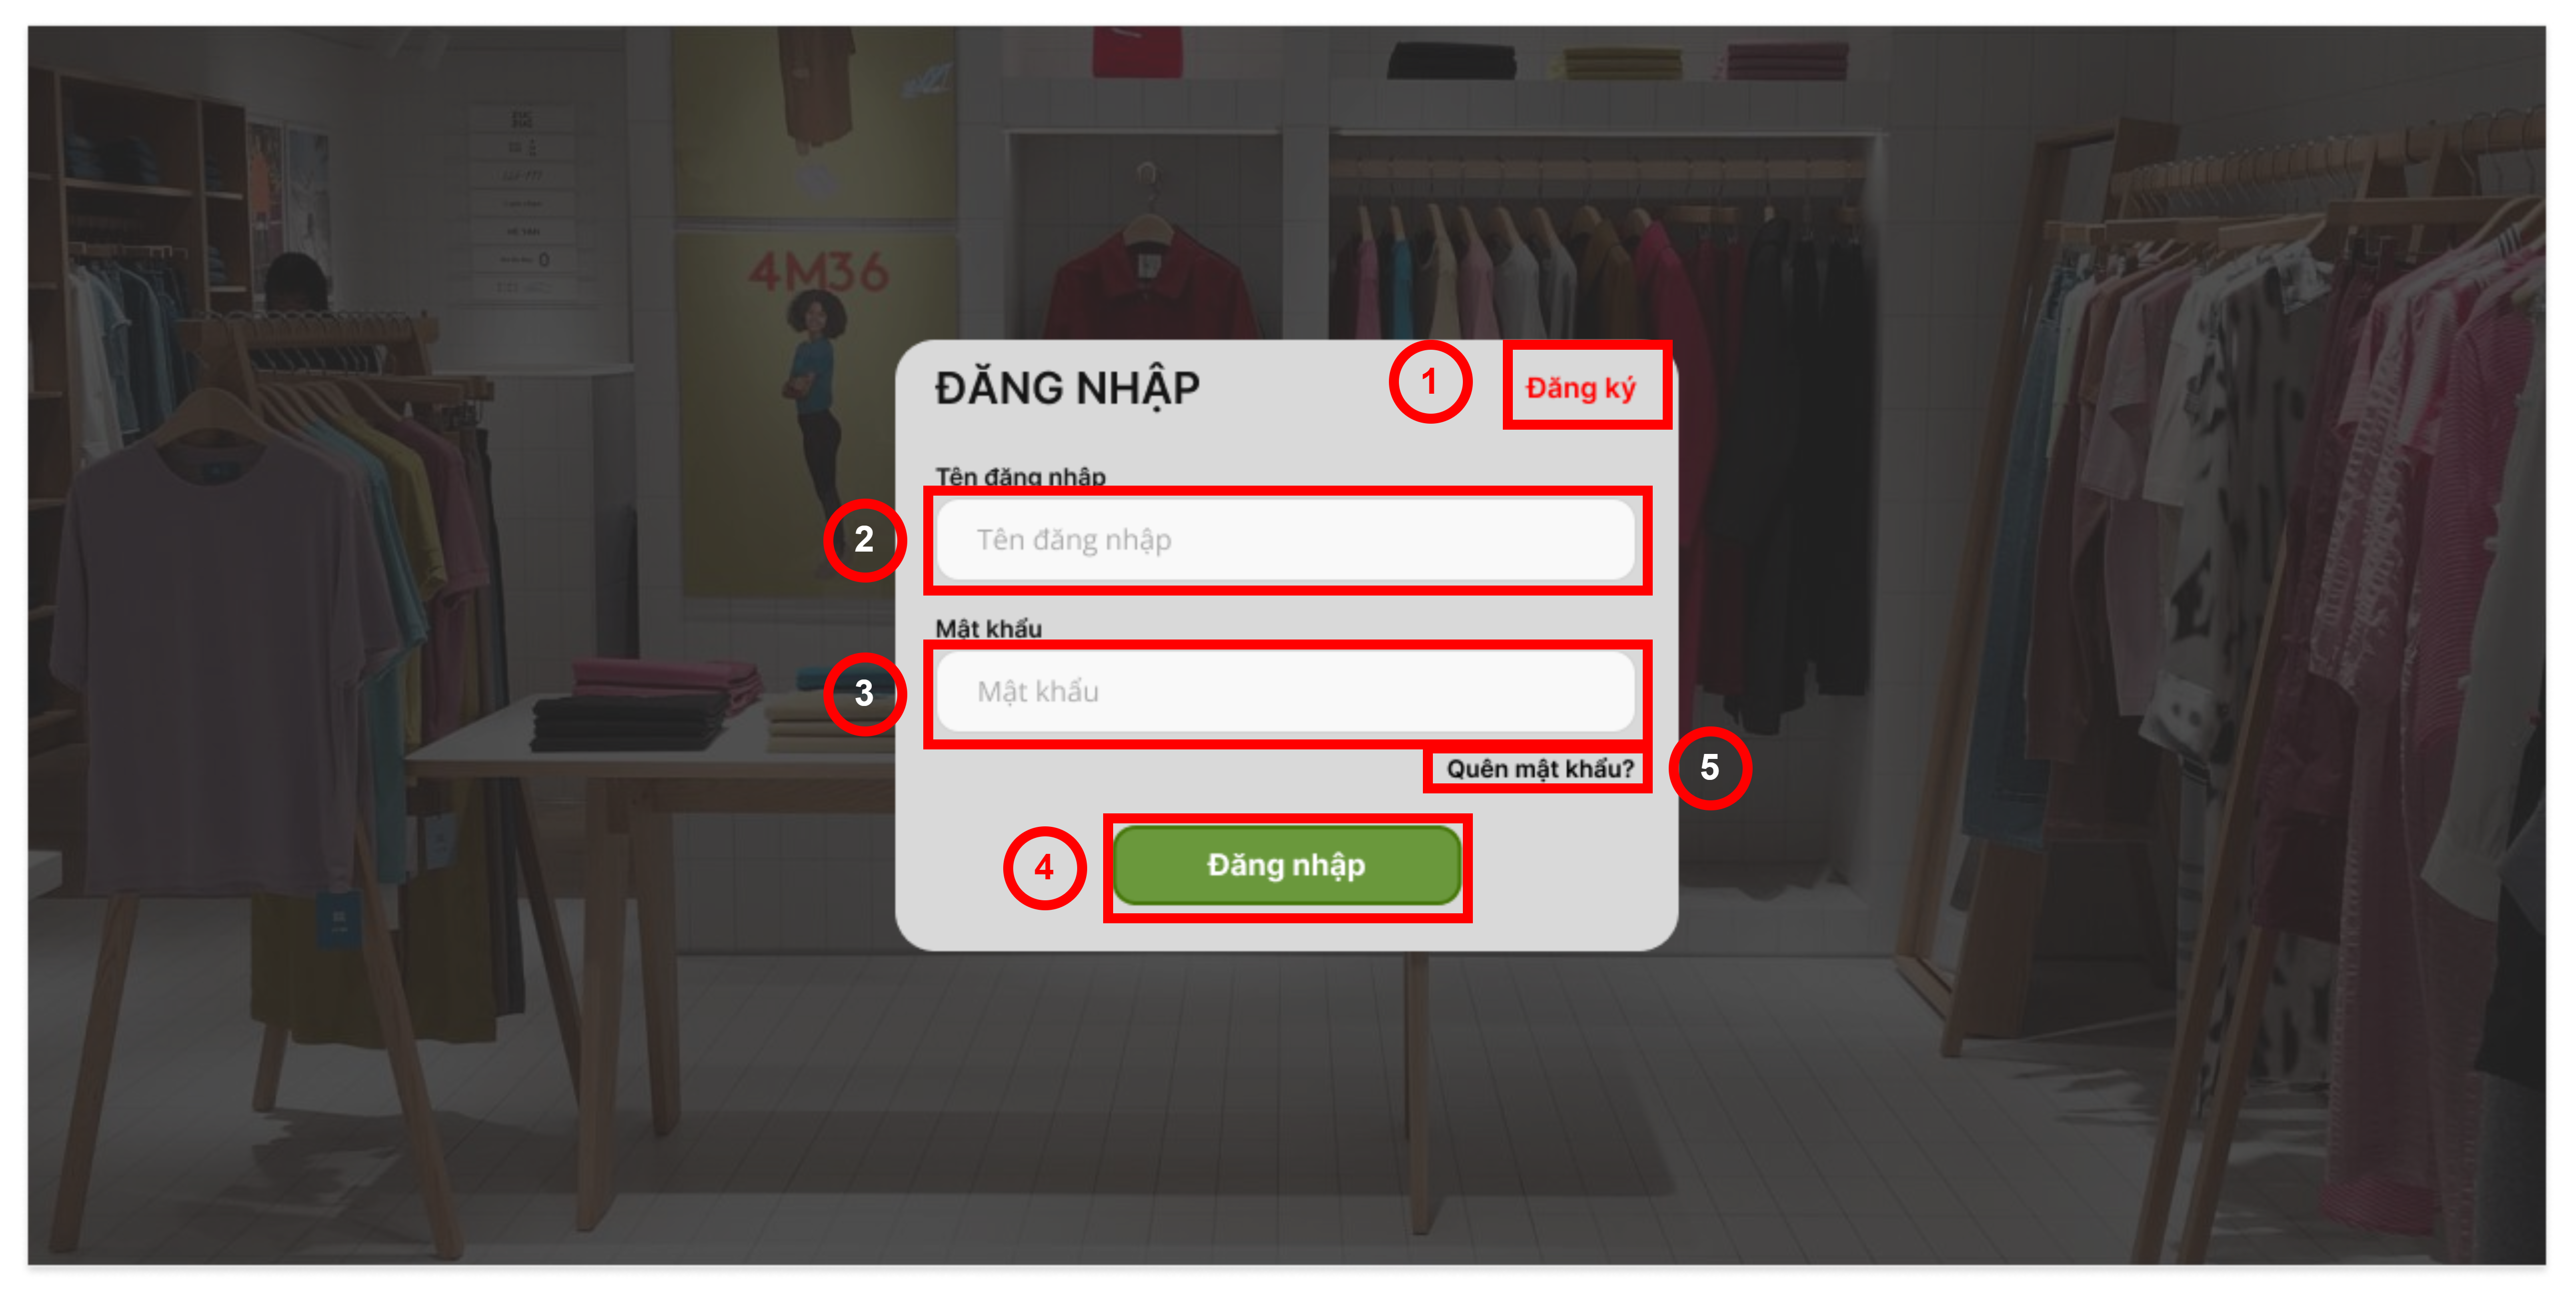
\includegraphics[width=5in]{img/UI/customer/login.png}
    \label{1}
    \newline
    \caption{Giao diện đăng nhập}
\end{figure}
\textbf{Mô tả:}
\begin{quote}
    \begin{enumerate}
        \item Chọn để chuyển tới trang đăng ký tài khoản.
        \item Nhập tên đăng nhập của tài khoản, yêu cầu tối thiểu 1 ký tự.
        \item Nhập mật khẩu của tài khoản, yêu cầu mật khẩu tối thiểu 6 ký tự.
        \item Chọn để thực hiện đăng nhập tài khoản, nếu thông tin tài khoản đúng thì sẽ được đưa đến giao diện mặc định cho tài khoản.
        \item Chọn "Quên mật khẩu" khi không nhớ mật khẩu của tài khoản để chuyển trang sang trang lấy lại mật khẩu.
    \end{enumerate}
\end{quote}


\subsection{Giao diện người dùng}
\subsubsection{Đăng ký}
\begin{figure}[!htp]
    \centering
    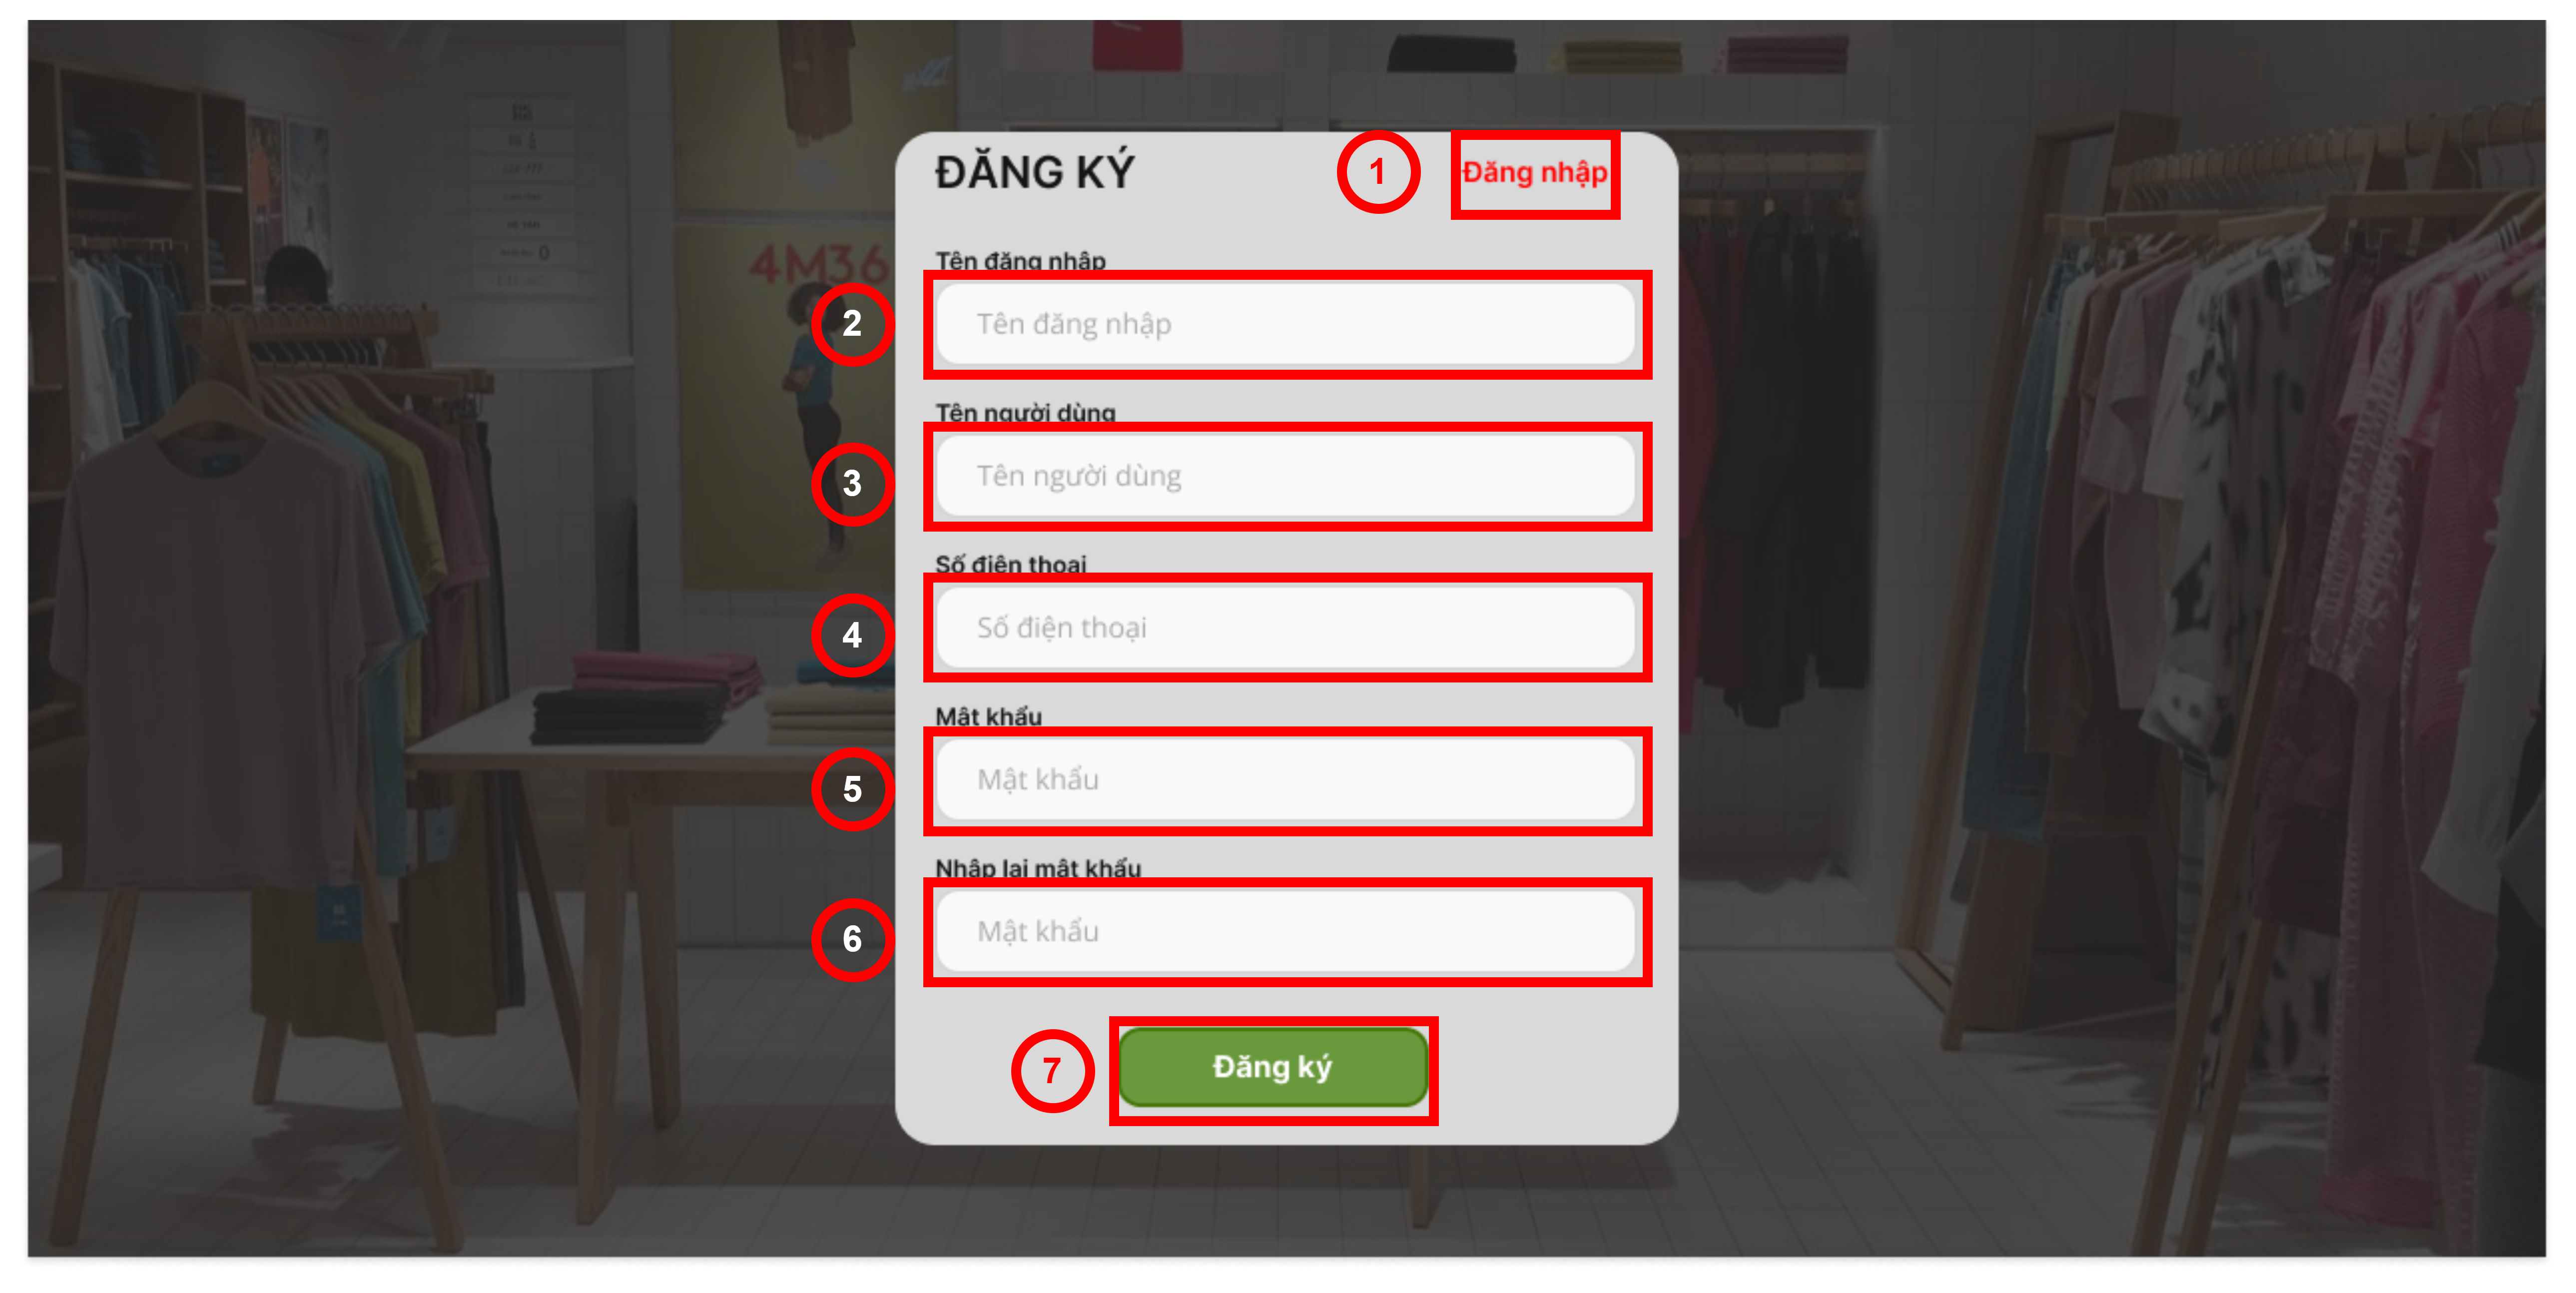
\includegraphics[width=5in]{img/UI/customer/register.png}
    \label{2}
    \newline
    \caption{Giao diện đăng ký tài khoản người dùng}
\end{figure}
\textbf{Mô tả:}
\begin{quote}
    \begin{enumerate}
        \item Chọn để chuyển tới trang đăng đăng nhập.
        \item Nhập tên đăng nhập của tài khoản, yêu cầu tối thiểu một ký tự.
        \item Nhập tên của người dùng, yêu cầu tối thiểu một ký tự.
        \item Nhập số điện thoại của người dùng, yêu cầu đúng định dạng số điện thoại 10 chữ số, bắt đầu bằng số 09 / 03 / 05 / 07 / 08.
        \item Nhập mật khẩu của tài khoản, yêu cầu tối thiểu 6 ký tự.
        \item Nhập lại mật khẩu của tài khoản, yêu cầu phải giống mật khẩu của tài khoản đã nhập.
        \item Chọn để thực hiện đăng ký tài khoản, nếu đăng ký thành công thì chuyển tới trang đăng nhập.
    \end{enumerate}
\end{quote}


\subsubsection{Tạo lại mật khẩu}
\begin{figure}[!htp]
    \centering
    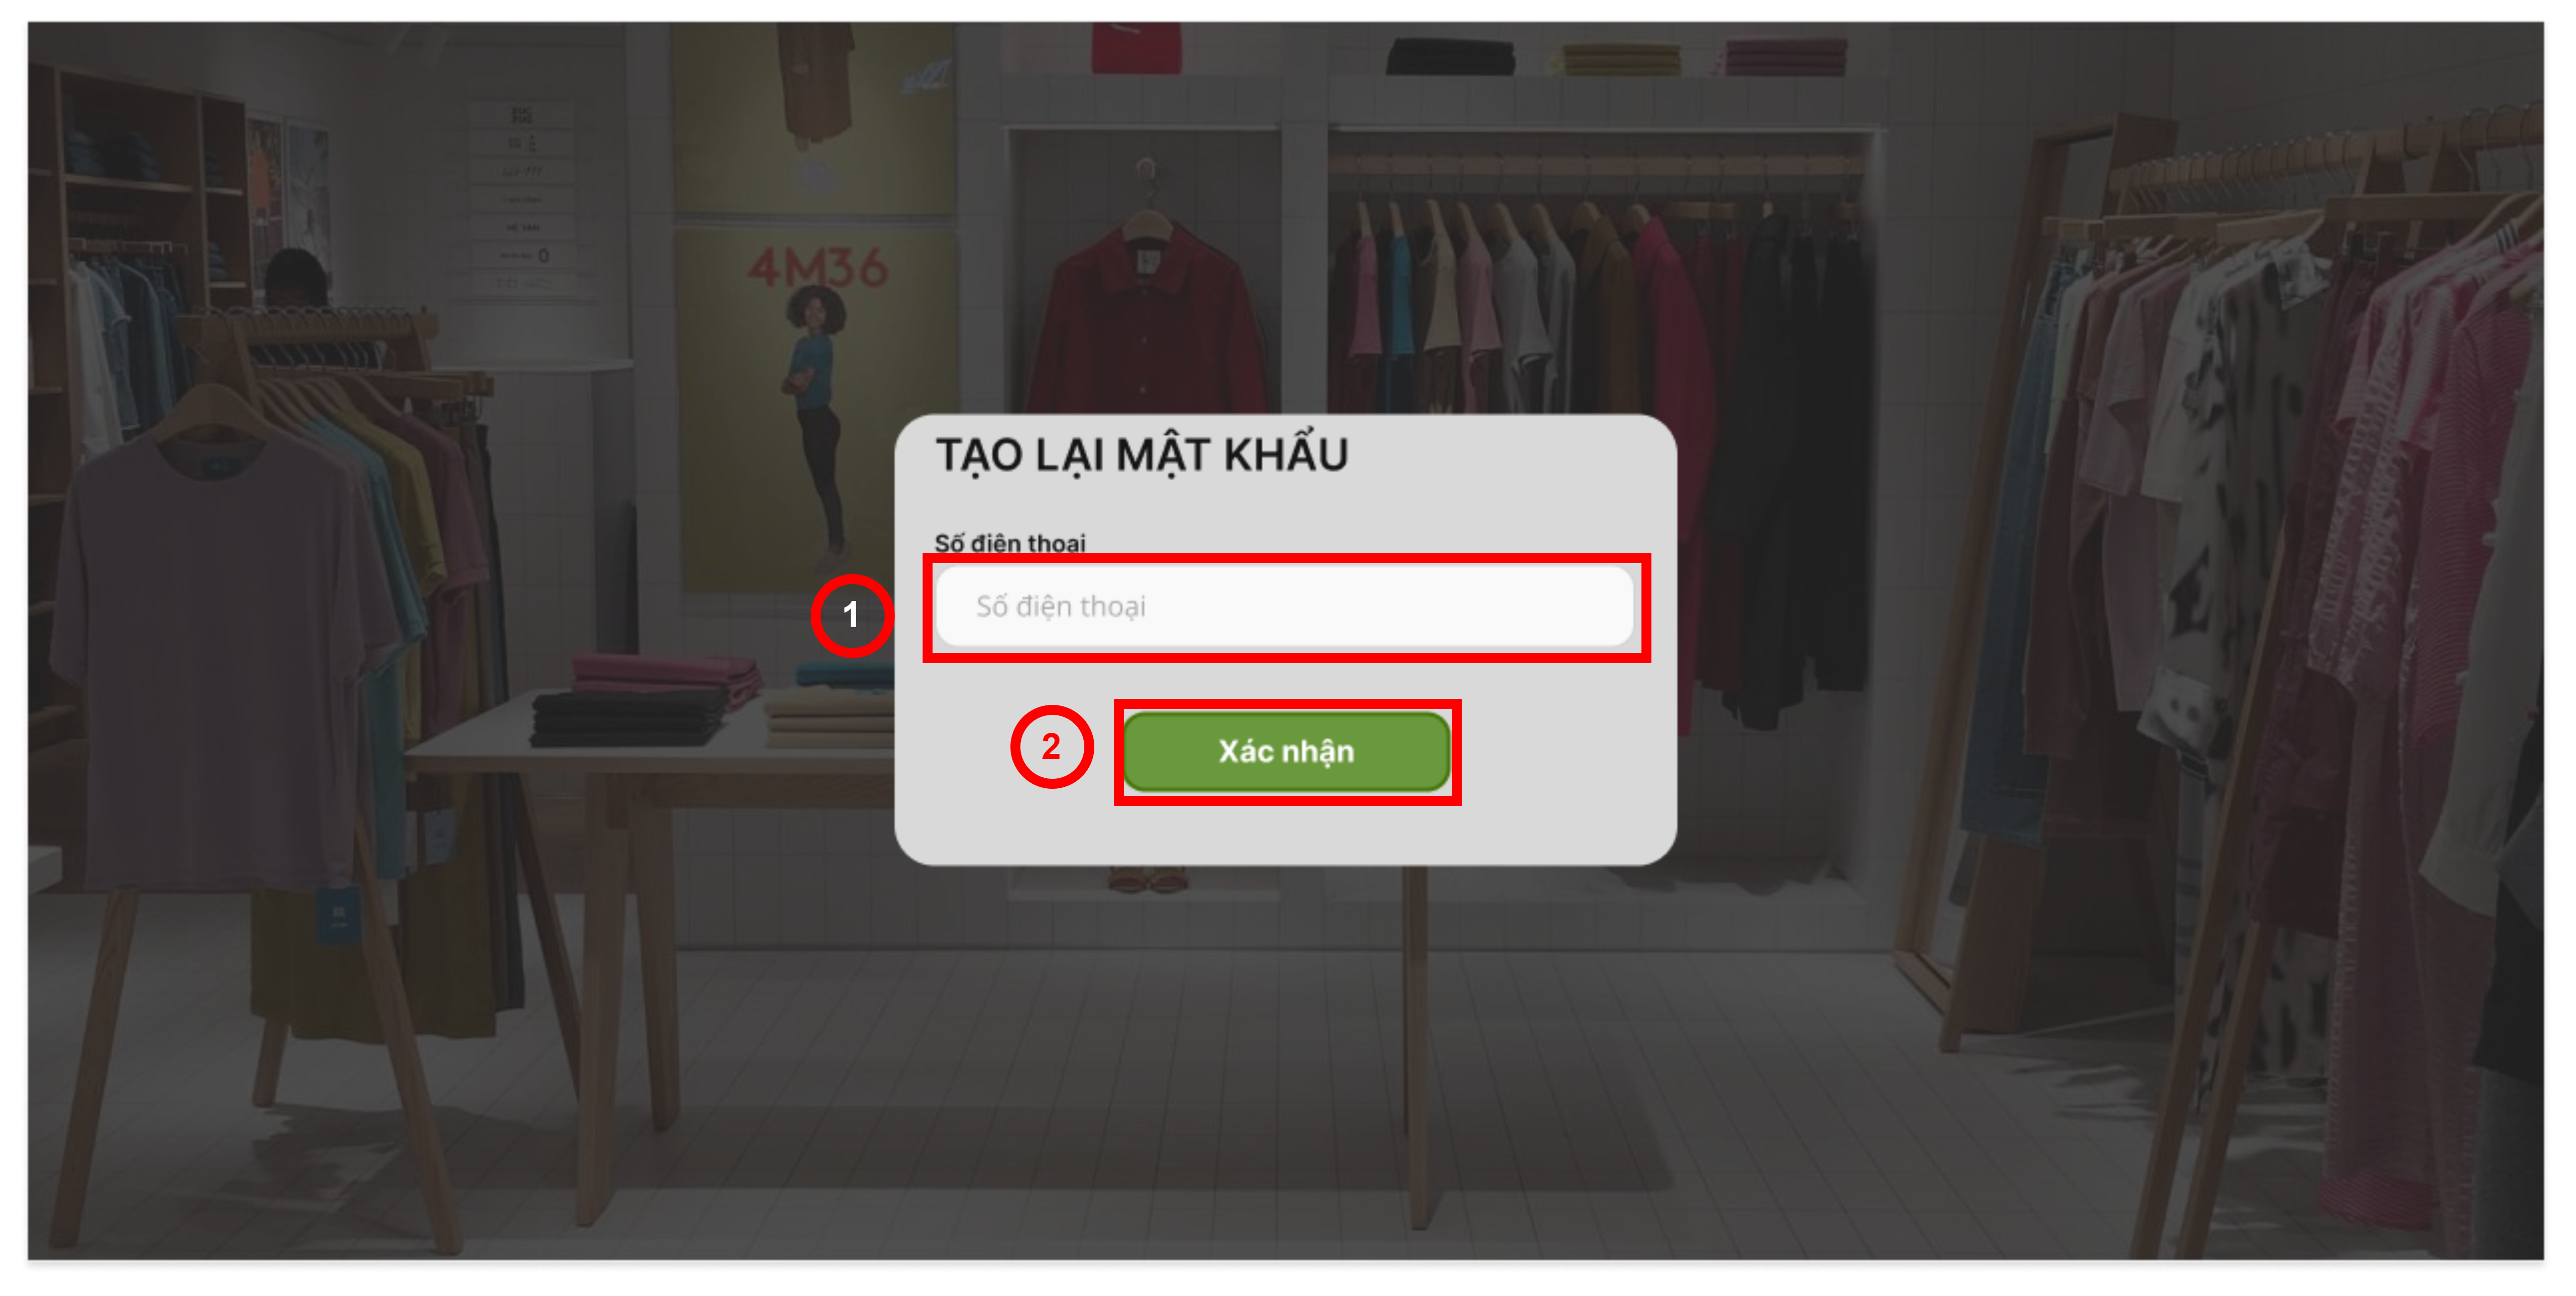
\includegraphics[width=5in]{img/UI/customer/reset_new_password.png}
    \label{3}
    \newline
    \caption{Giao diện tạo lại mật khẩu người dùng}
\end{figure}
\textbf{Mô tả:}
\begin{quote}
    \begin{enumerate}
        \item Người dùng nhập số điện thoại của tài khoản, yêu cầu đúng định dạng số điện thoại 10 chữ số, bắt đầu bằng số 09 / 03 / 05 / 07 / 08.
        \item Người dùng chọn để hệ thống gửi xác nhận tin nhắn OTP và chuyển tới trang xác nhận OTP.
    \end{enumerate}
\end{quote}
\newpage
\begin{figure}[!htp]
    \centering
    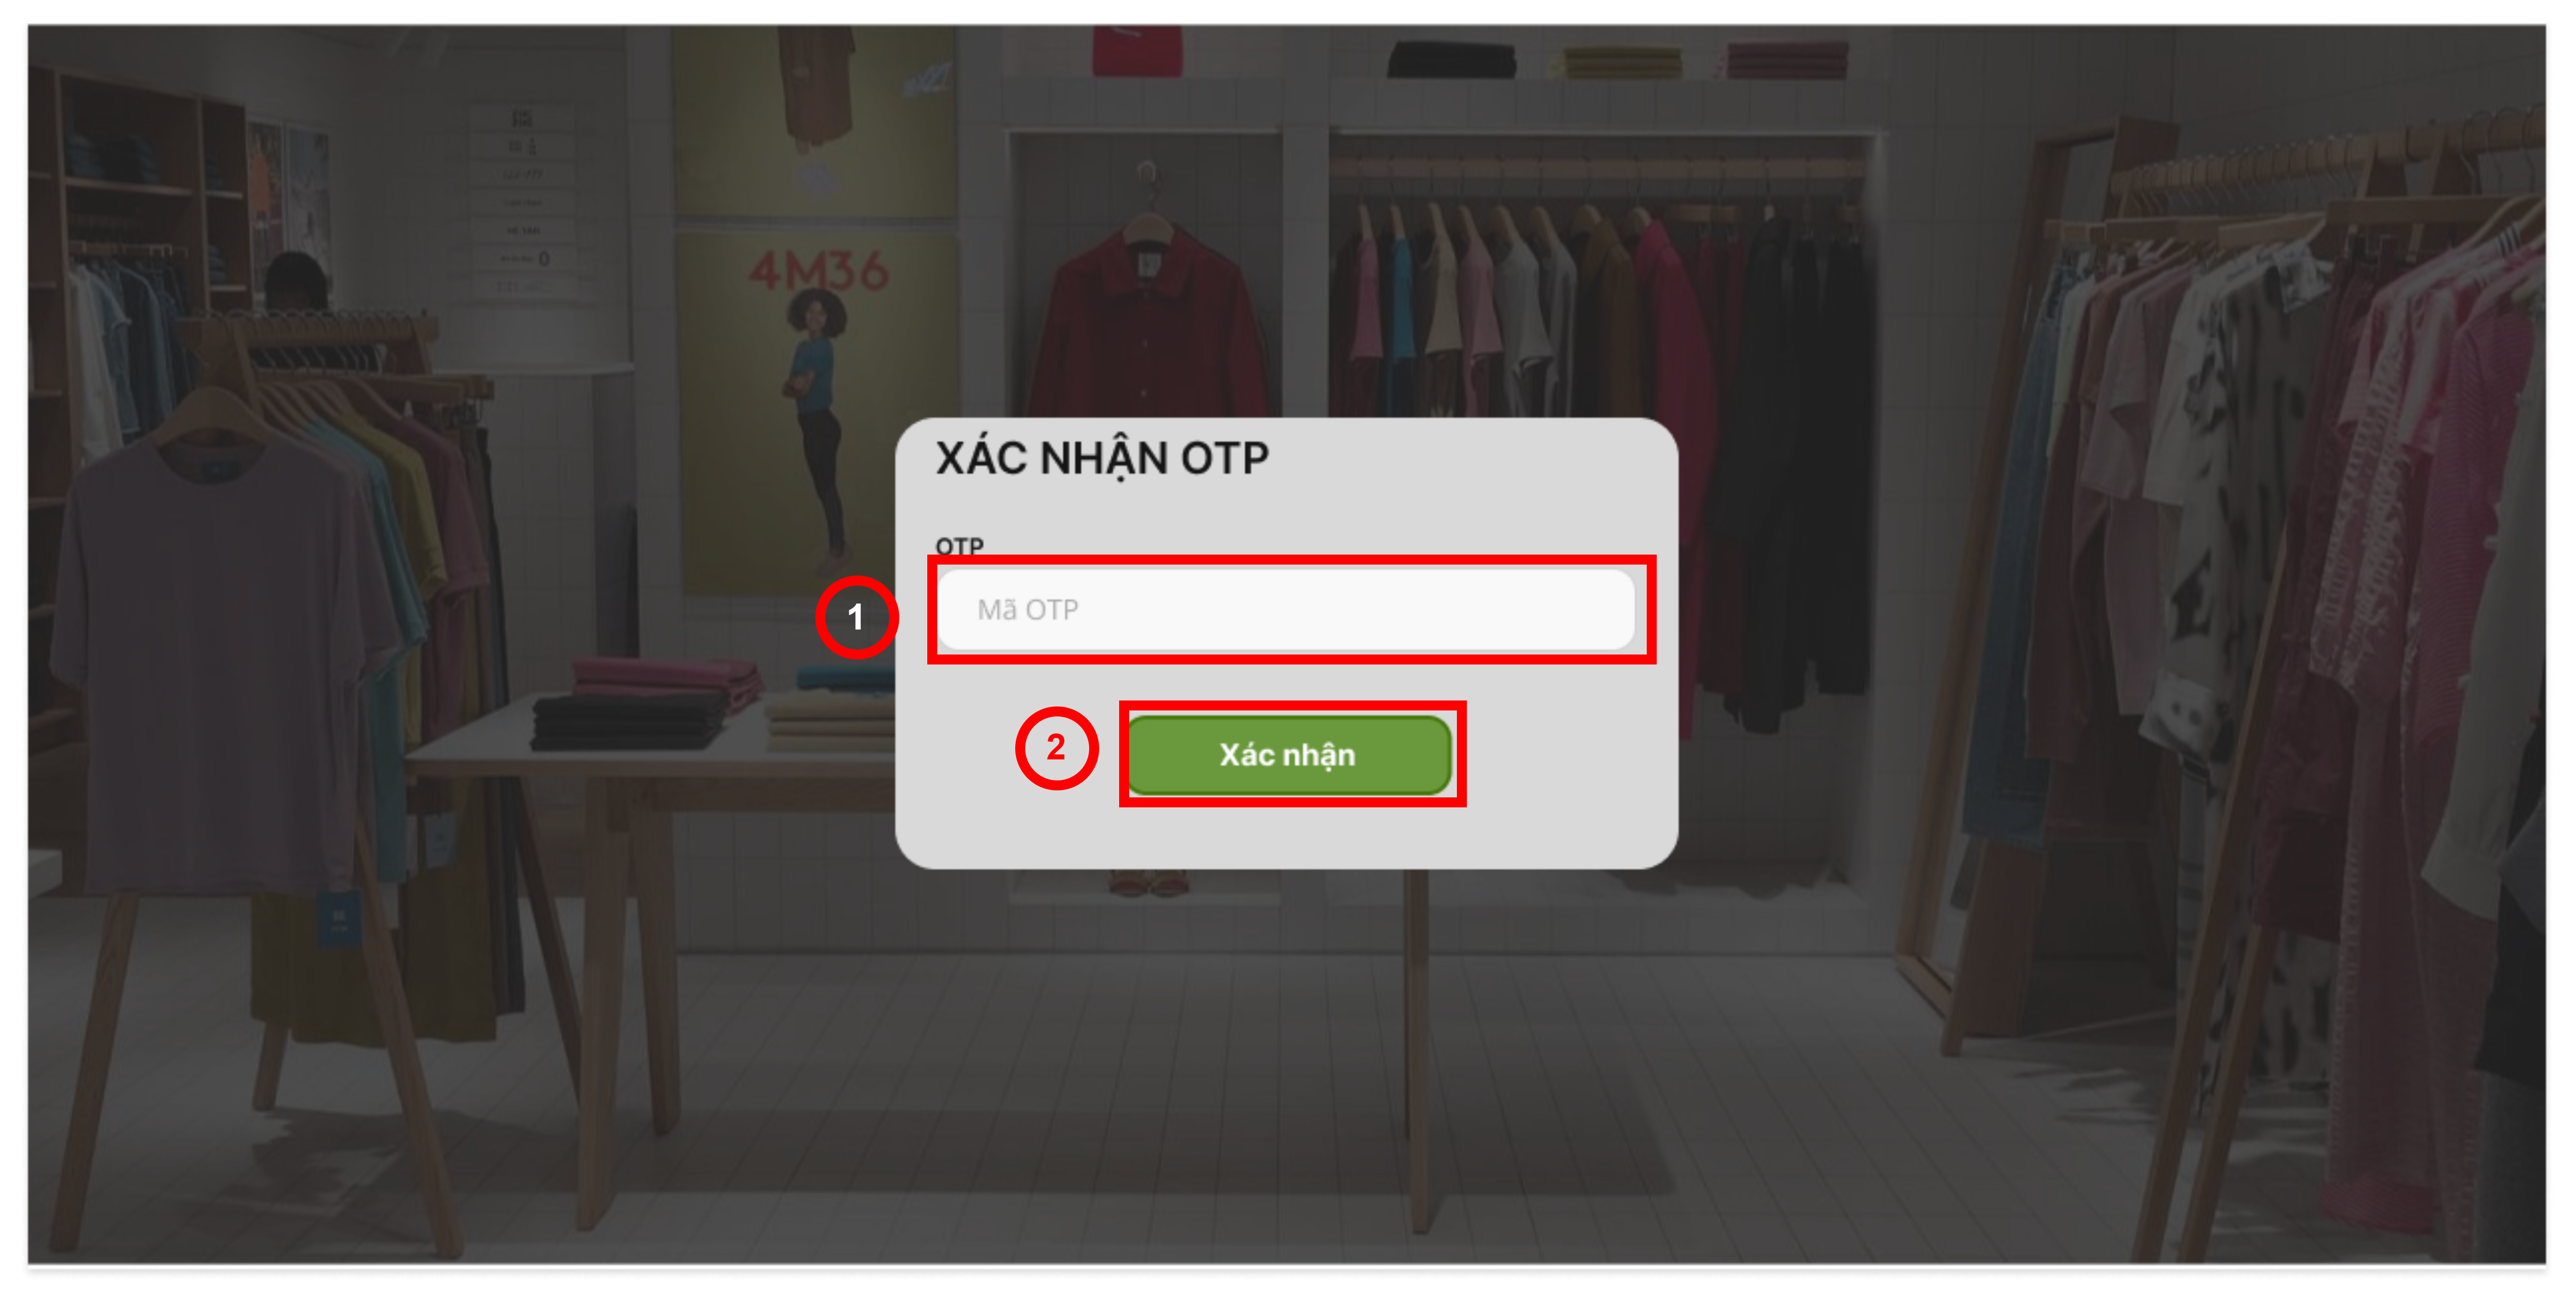
\includegraphics[width=5in]{img/UI/customer/confirm_otp.png}
    \label{4}
    \newline
    \caption{Giao diện xác nhận OTP}
\end{figure}
\textbf{Mô tả:}
\begin{quote}
    \begin{enumerate}
        \item Người dùng nhập OTP đã được gửi qua tin nhắn, yêu cầu 6 ký tự.
        \item Người dùng chọn để hệ thống xác nhận và thông tin hợp lệ sẽ được chuyển đến trang tạo lại mật khẩu mới.
    \end{enumerate}
\end{quote}
\textbf{Mô tả:}
\begin{quote}
    \begin{enumerate}
        \item Người dùng nhập số điện thoại của tài khoản, yêu cầu đúng định dạng số điện thoại 10 chữ số, bắt đầu bằng số 09 / 03 / 05 / 07 / 08.
        \item Người dùng chọn để hệ thống gửi xác nhận tin nhắn OTP và chuyển tới trang xác nhận OTP.
    \end{enumerate}
\end{quote}
\begin{figure}[!htp]
    \centering
    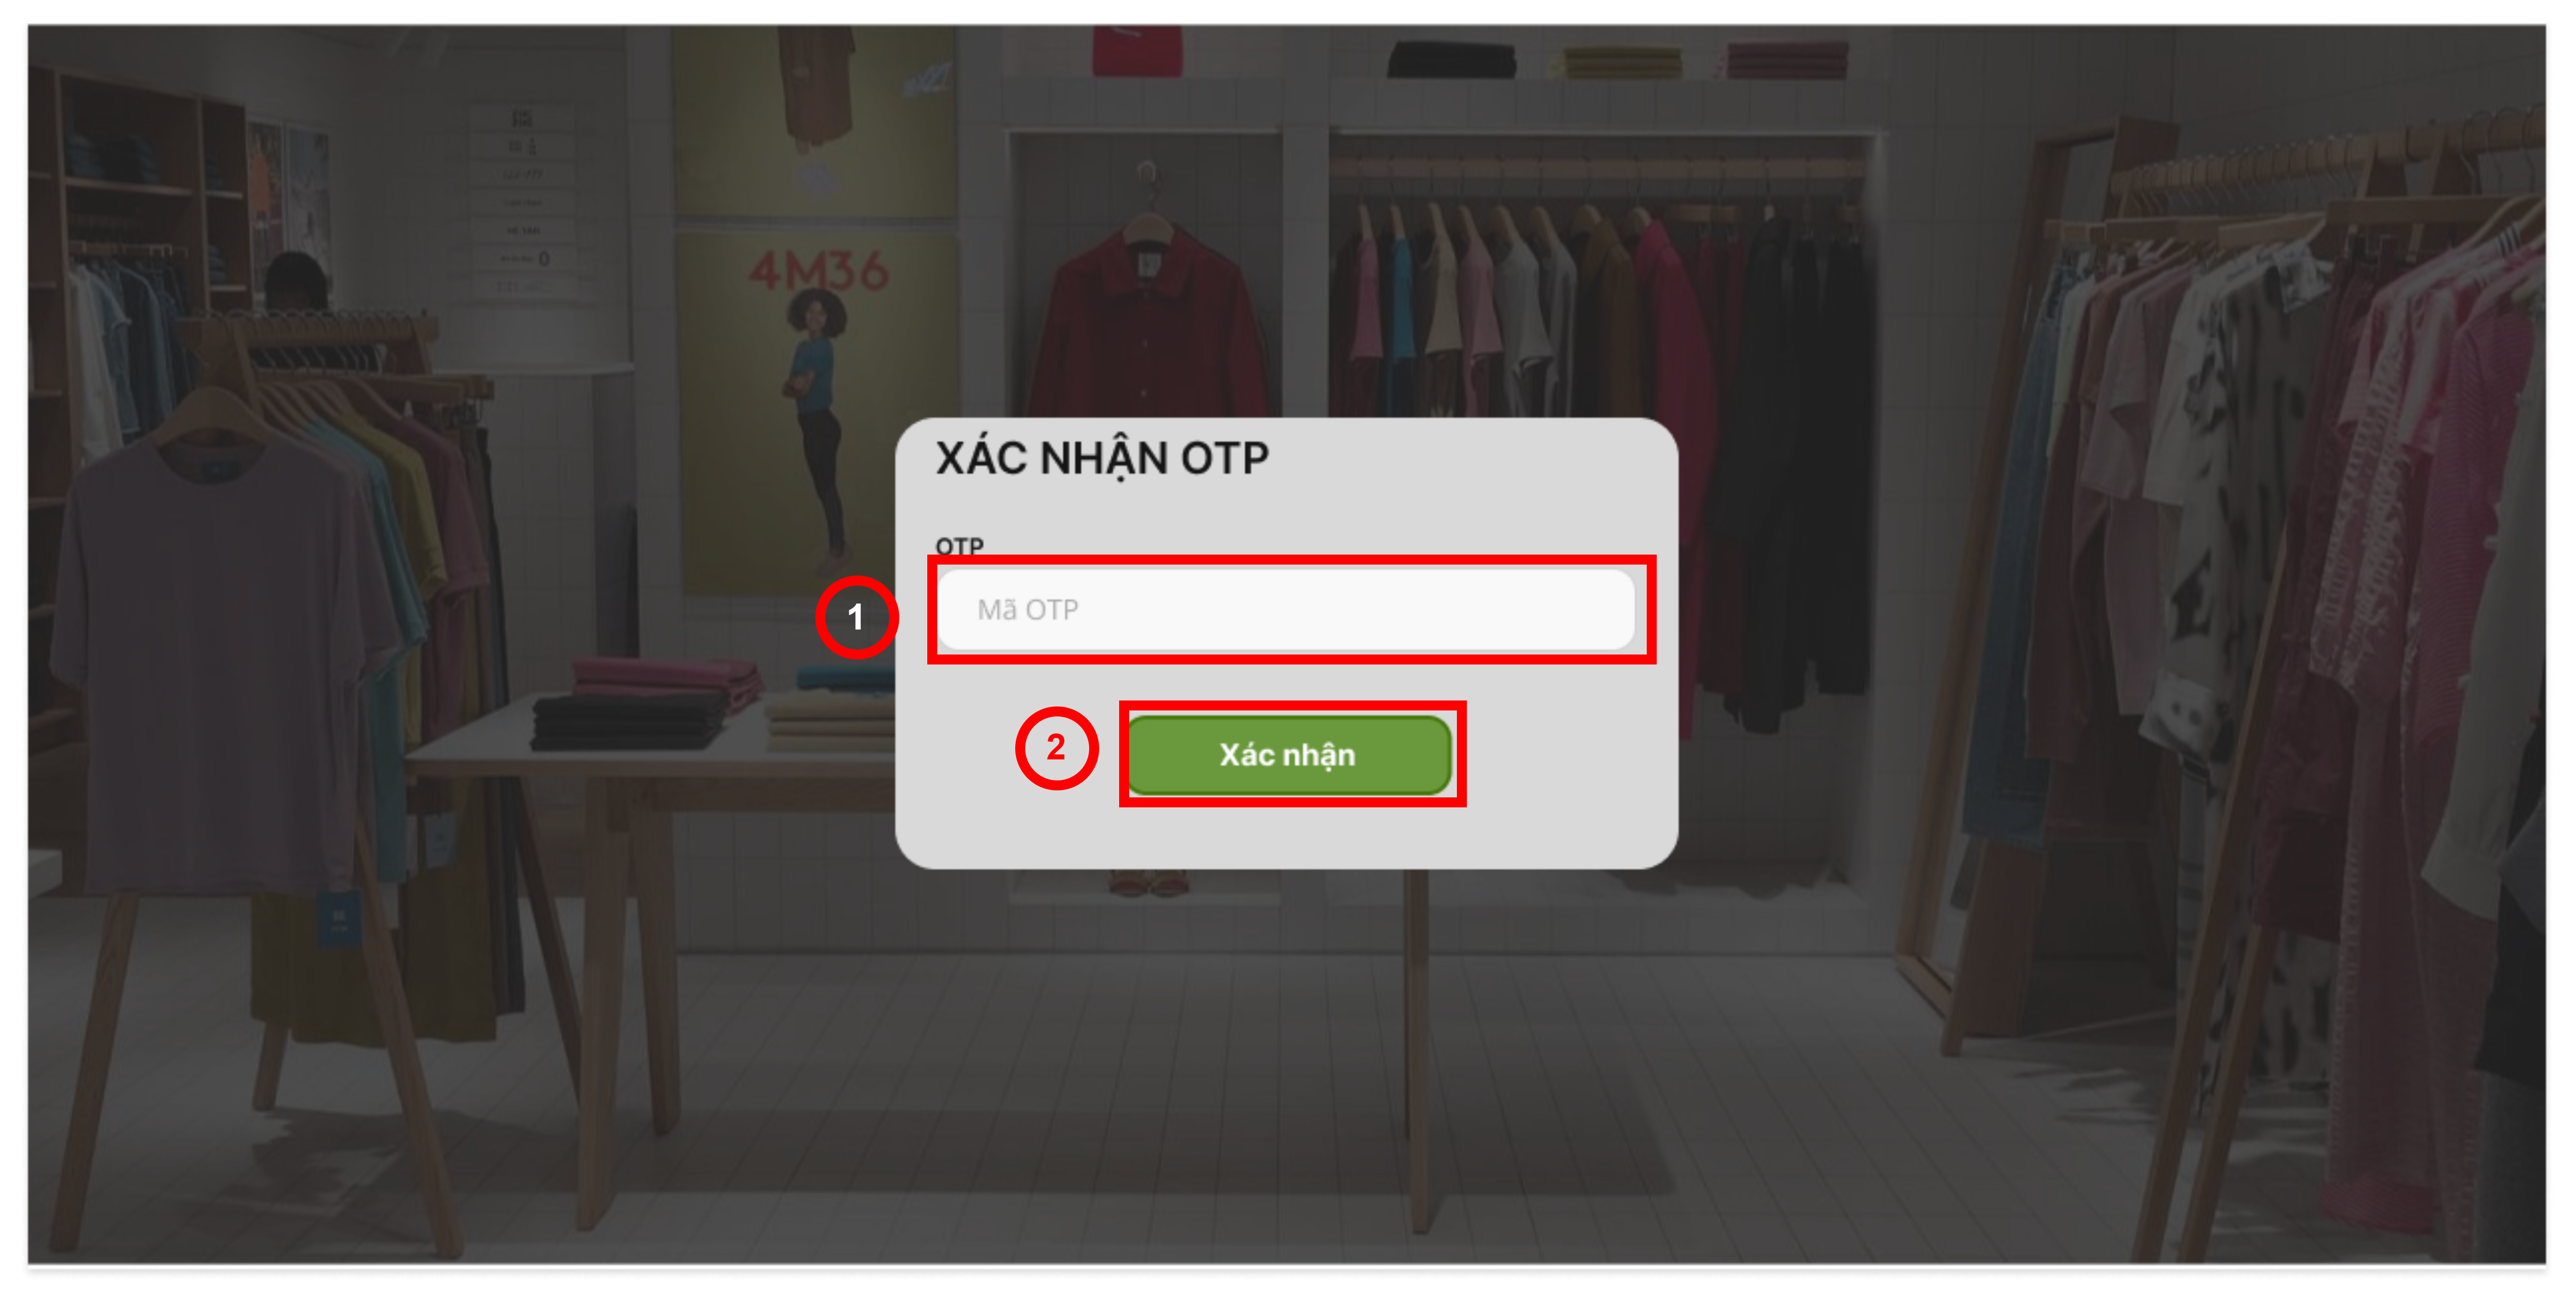
\includegraphics[width=5in]{img/UI/customer/confirm_otp.png}
    \label{5}
    \newline
    \caption{Giao diện tạo lại mật khẩu mới}
\end{figure}
\textbf{Mô tả:}
\begin{quote}
    \begin{enumerate}
        \item Người dùng nhập mật khẩu mới cho tài khoản, yêu cầu tối thiểu 6 ký tự.
        \item Người dùng nhập lại mật khẩu mới cho tài khoản, yêu cầu phải giống với mật khẩu mới.
        \item Người dùng chọn "Xác nhận" để cập nhật lại mật khẩu mới cho tài khoản.
    \end{enumerate}
\end{quote}

\subsubsection{Header}
\begin{figure}[!htp]
    \centering
    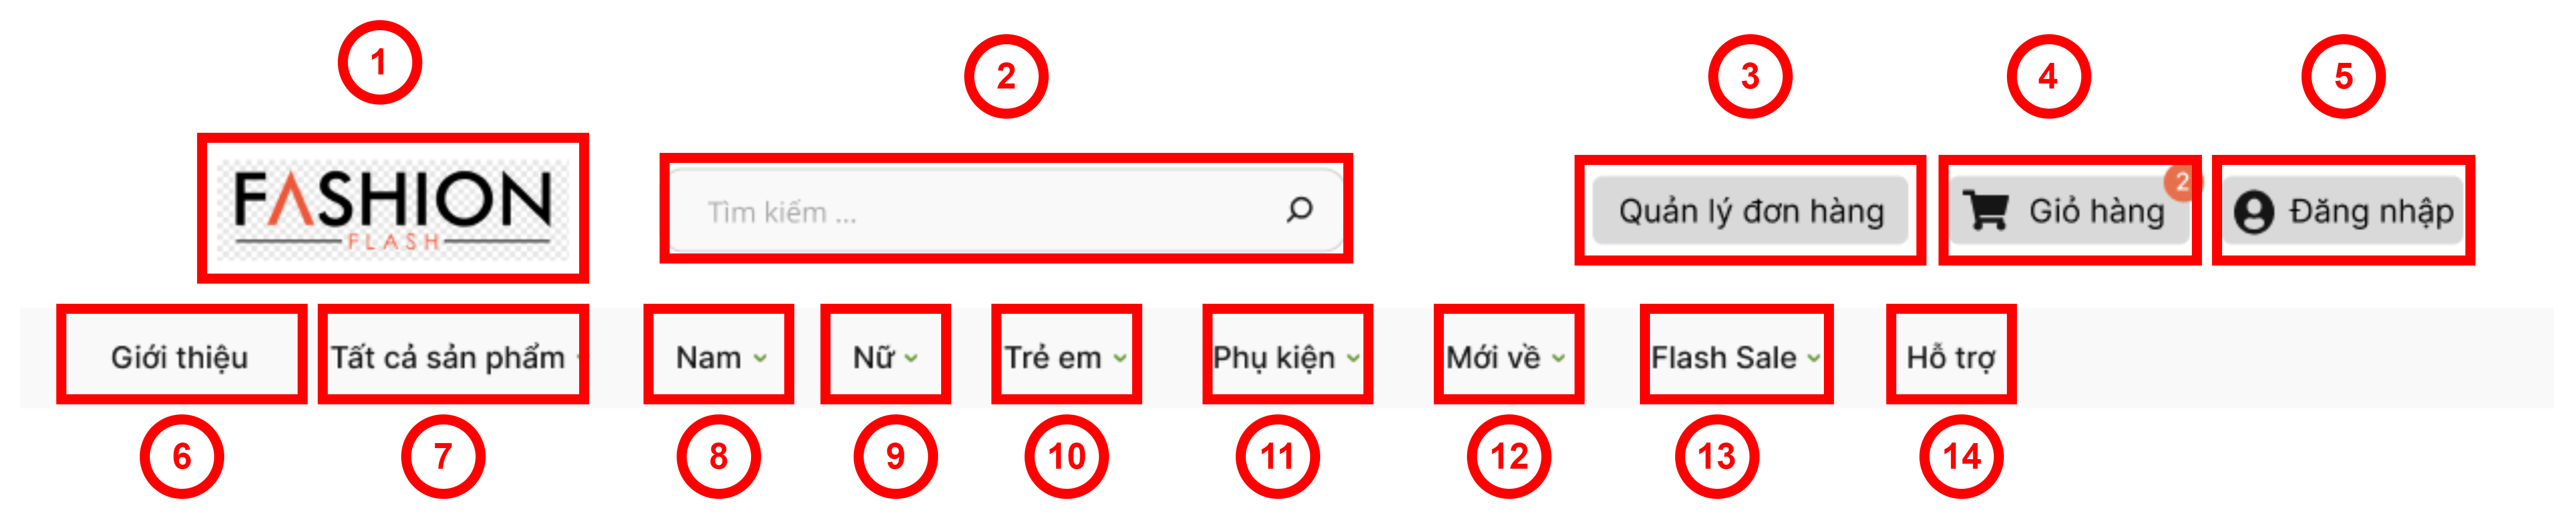
\includegraphics[width=5in]{img/UI/customer/header.png}
    \label{6}
    \newline
    \caption{Giao diện phần header}
\end{figure}
\textbf{Mô tả:}
\begin{quote}
    \begin{enumerate}
        \item Chọn để chuyển tới trang chủ.
        \item Nhập tên sản phẩm cần tìm và nhấn enter để tìm kiếm sản phẩm.
        \item Chọn để chuyển đến trang quản lý lịch sử đơn hàng đã thực hiện.
        \item Chọn để chuyển đến trang quản lý giỏ hàng.
        \item Chọn để đăng nhập.
        \item Chọn để chuyển đến trang giới thiệu về hệ thống cửa hàng.
        \item Chọn để chuyển đến trang tất cả sản phẩm.
        \item Chọn để chuyển đến trang tất cả sản phẩm với lựa chọn lọc sẵn là sản phẩm dành cho nam.
        \item Chọn để chuyển đến trang tất cả sản phẩm với lựa chọn lọc sẵn là sản phẩm dành cho nữ.
        \item Chọn để chuyển đến trang tất cả sản phẩm với lựa chọn lọc sẵn là sản phẩm dành cho trẻ em.
        \item Chọn để chuyển đến trang tất cả sản phẩm với lựa chọn lọc sẵn là sản phẩm thuộc dòng phụ kiện.
        \item Chọn để chuyển đến trang các sản phẩm mới về.
        \item Chọn để chuyển đến trang các sản phẩm đang được flash sale.
        \item Chọn để chuyển đến trang hỗ trợ cho khách hàng.
    \end{enumerate}
\end{quote}

\subsubsection{Footer}
\begin{figure}[!htp]
    \centering
    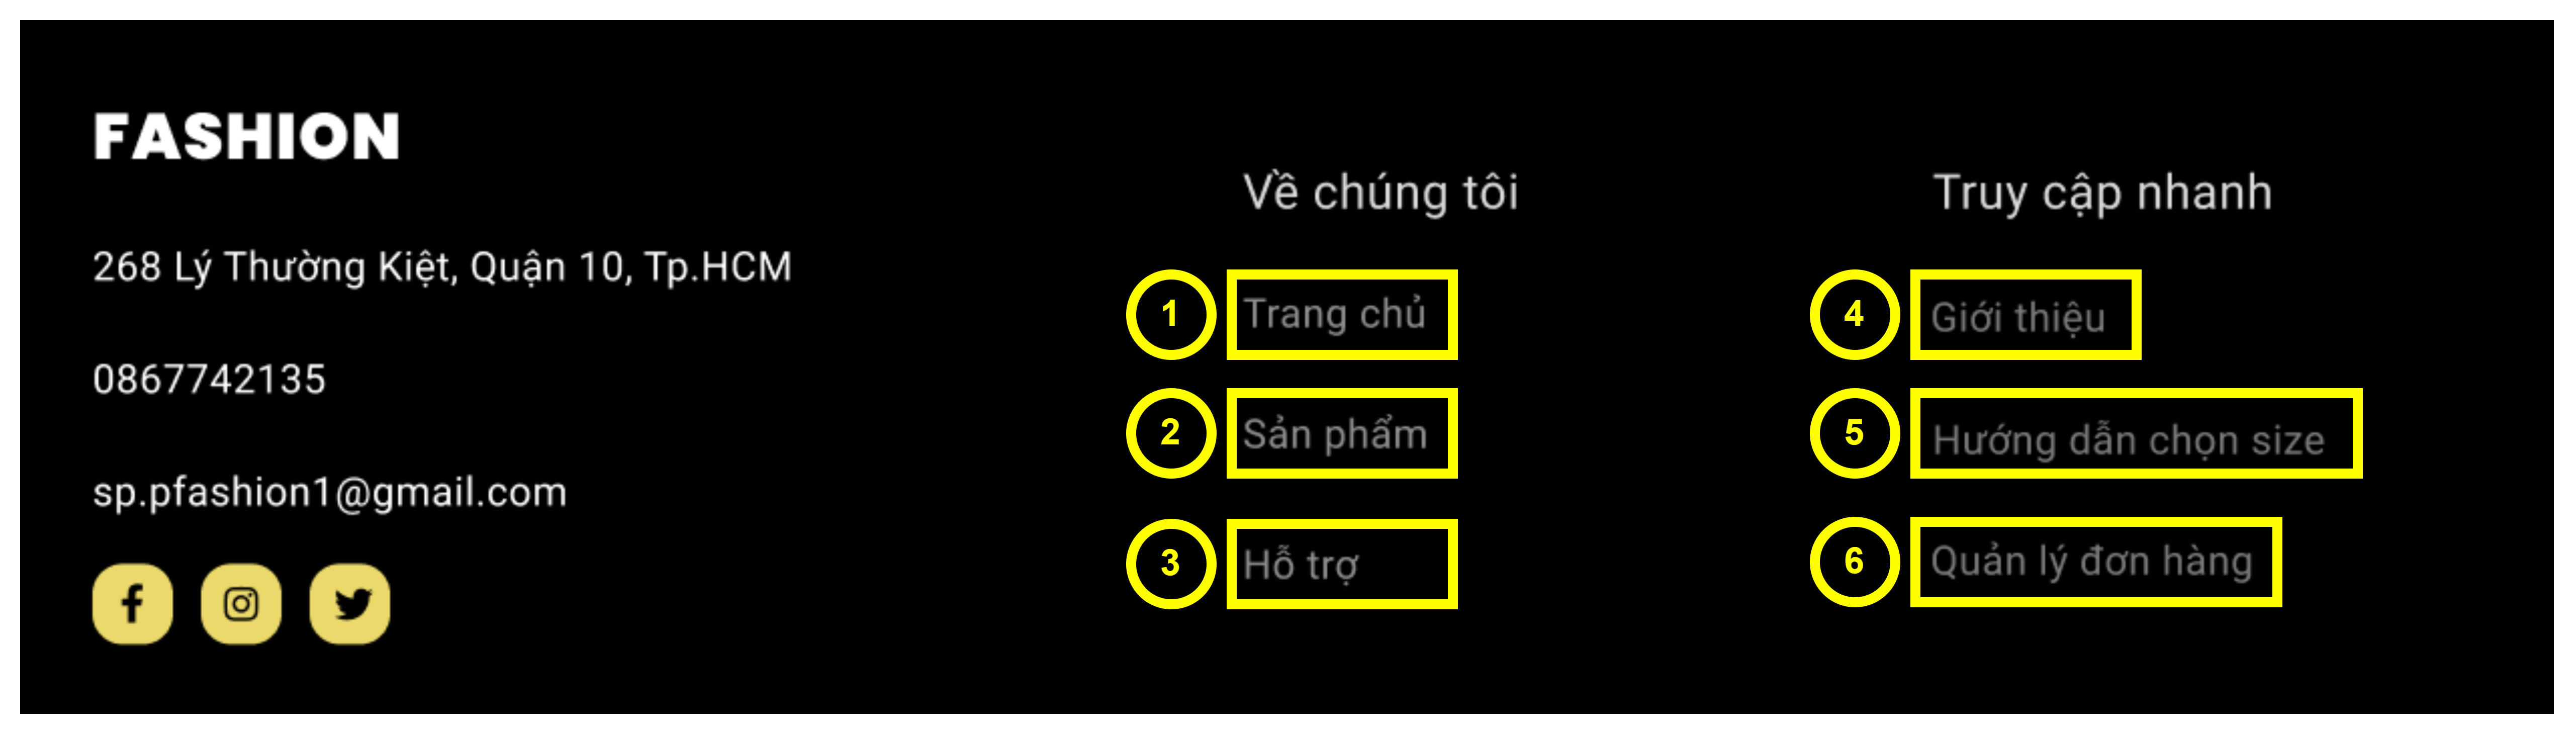
\includegraphics[width=5in]{img/UI/customer/footer.png}
    \label{7}
    \newline
    \caption{Giao diện phần footer}
\end{figure}
\textbf{Mô tả:}
\begin{quote}
    \begin{enumerate}
        \item Chọn để chuyển tới trang chủ.
        \item Chọn để chuyển đến trang tất cả sản phẩm.
        \item Chọn để chuyển đến trang hỗ trợ cho khách hàng.
        \item Chọn để chuyển đến trang giới thiệu về hệ thống cửa hàng.
        \item Chọn để xem hướng dẫn chọn size.
        \item Chọn để chuyển đến trang quản lý lịch sử đơn hàng đã thực hiện.
    \end{enumerate}
\end{quote}

\newpage
\subsubsection{Trang chủ}
\begin{figure}[!htp]
    \centering
    \includegraphics[width=3.5in]{img/UI/customer/home.png}
    \label{8}
    \newline
    \caption{Giao diện trang chủ khi người dùng truy cập vào trang web}
\end{figure}
\textbf{Mô tả:}
\begin{quote}
    \begin{enumerate}
        \item Chọn để xem thông tin chi tiết của sản phẩm.
        \item Chọn để thêm nhanh sản phẩm vào giỏ hàng.
    \end{enumerate}
\end{quote}

\subsubsection{Thông tin chi tiết sản phẩm}
\begin{figure}[!htp]
    \centering
    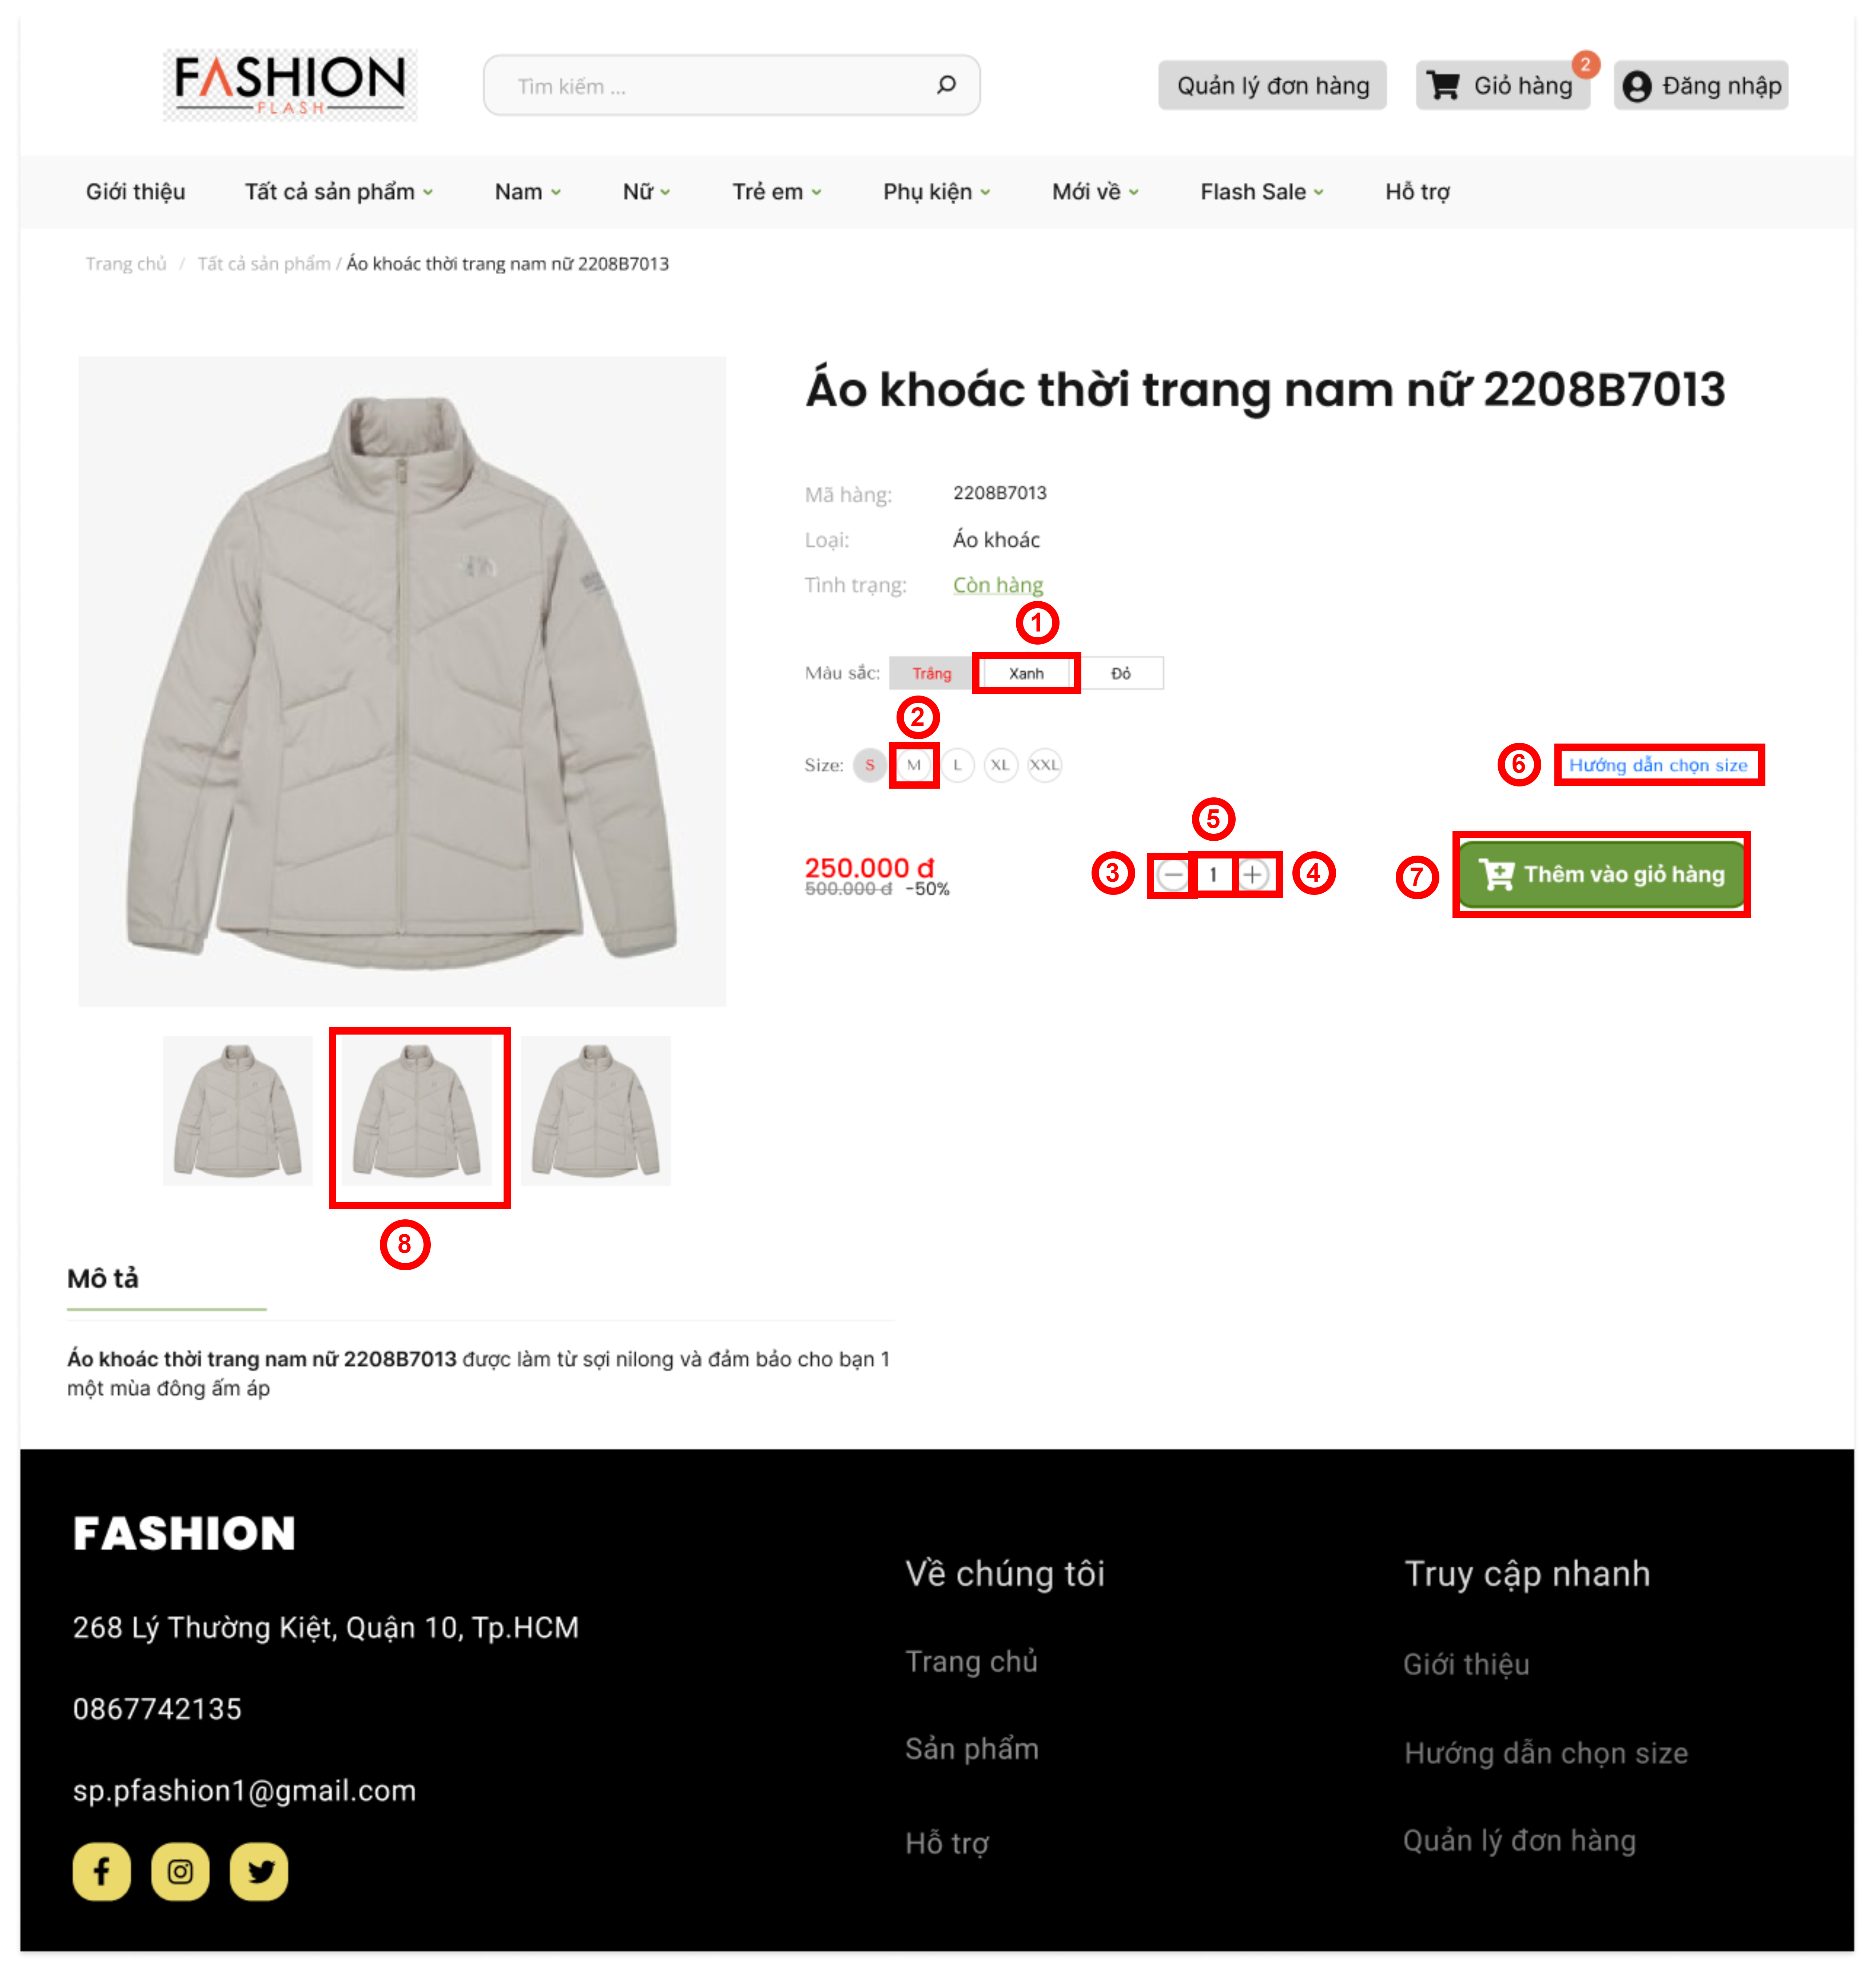
\includegraphics[width=5in]{img/UI/customer/product_detail.png}
    \label{9}
    \newline
    \caption{Giao diện thông tin chi tiết của sản phẩm}
\end{figure}
\textbf{Mô tả:}
\begin{quote}
    \begin{enumerate}
        \item Chọn màu của sản phẩm mà người dùng muốn.
        \item Chọn size của sản phẩm mà người dùng muốn.
        \item Chọn để giảm số lượng mà người dùng muốn.
        \item Chọn để tăng số lượng mà người dùng muốn.
        \item Nhập để thay đổi số lượng mà người dùng muốn.
        \item Chọn để xem hướng dẫn chọn size cho sản phẩm.
        \item Chọn để thêm sản phẩm với màu sắc, size và số lượng mà người dùng đã chọn.
        \item Chọn để xem ảnh chi tiết mà người dùng muốn.
    \end{enumerate}
\end{quote}

\begin{figure}[!htp]
    \centering
    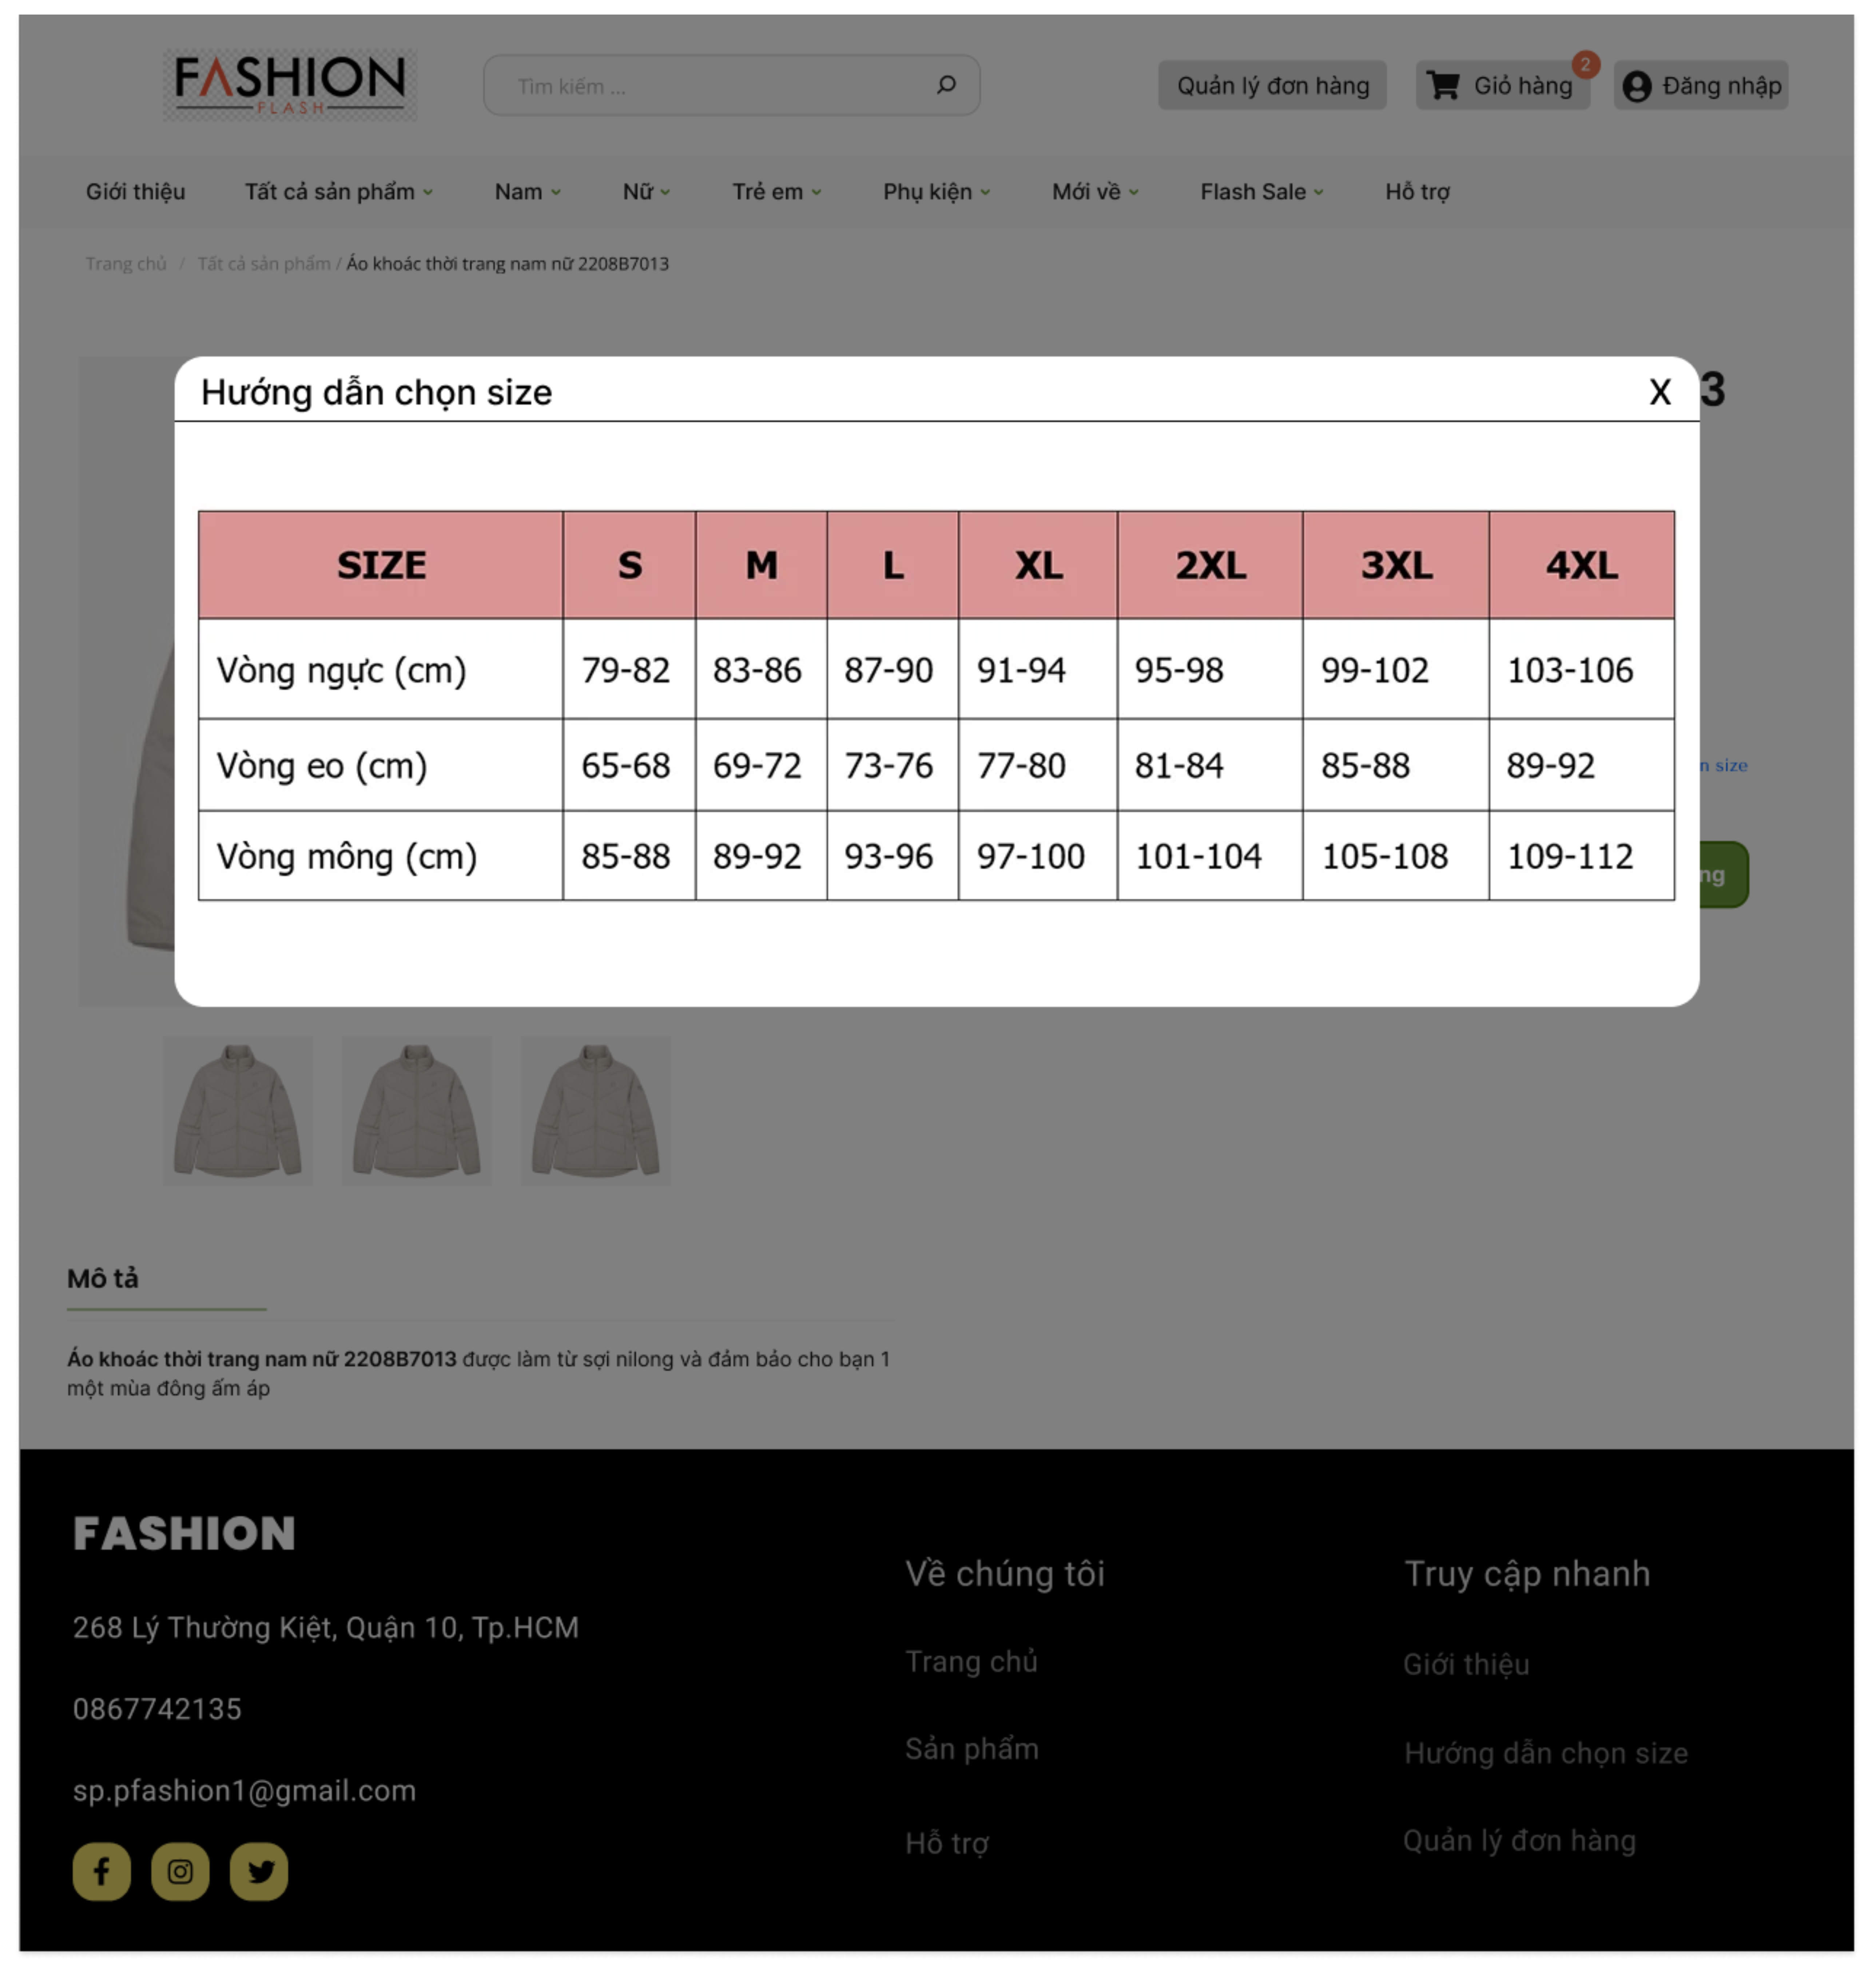
\includegraphics[width=5in]{img/UI/customer/guide_size.png}
    \label{10}
    \newline
    \caption{Giao diện hướng dẫn chọn size cho sản phẩm}
\end{figure}
\newpage

\subsubsection{Giỏ hàng}
\begin{figure}[!htp]
    \centering
    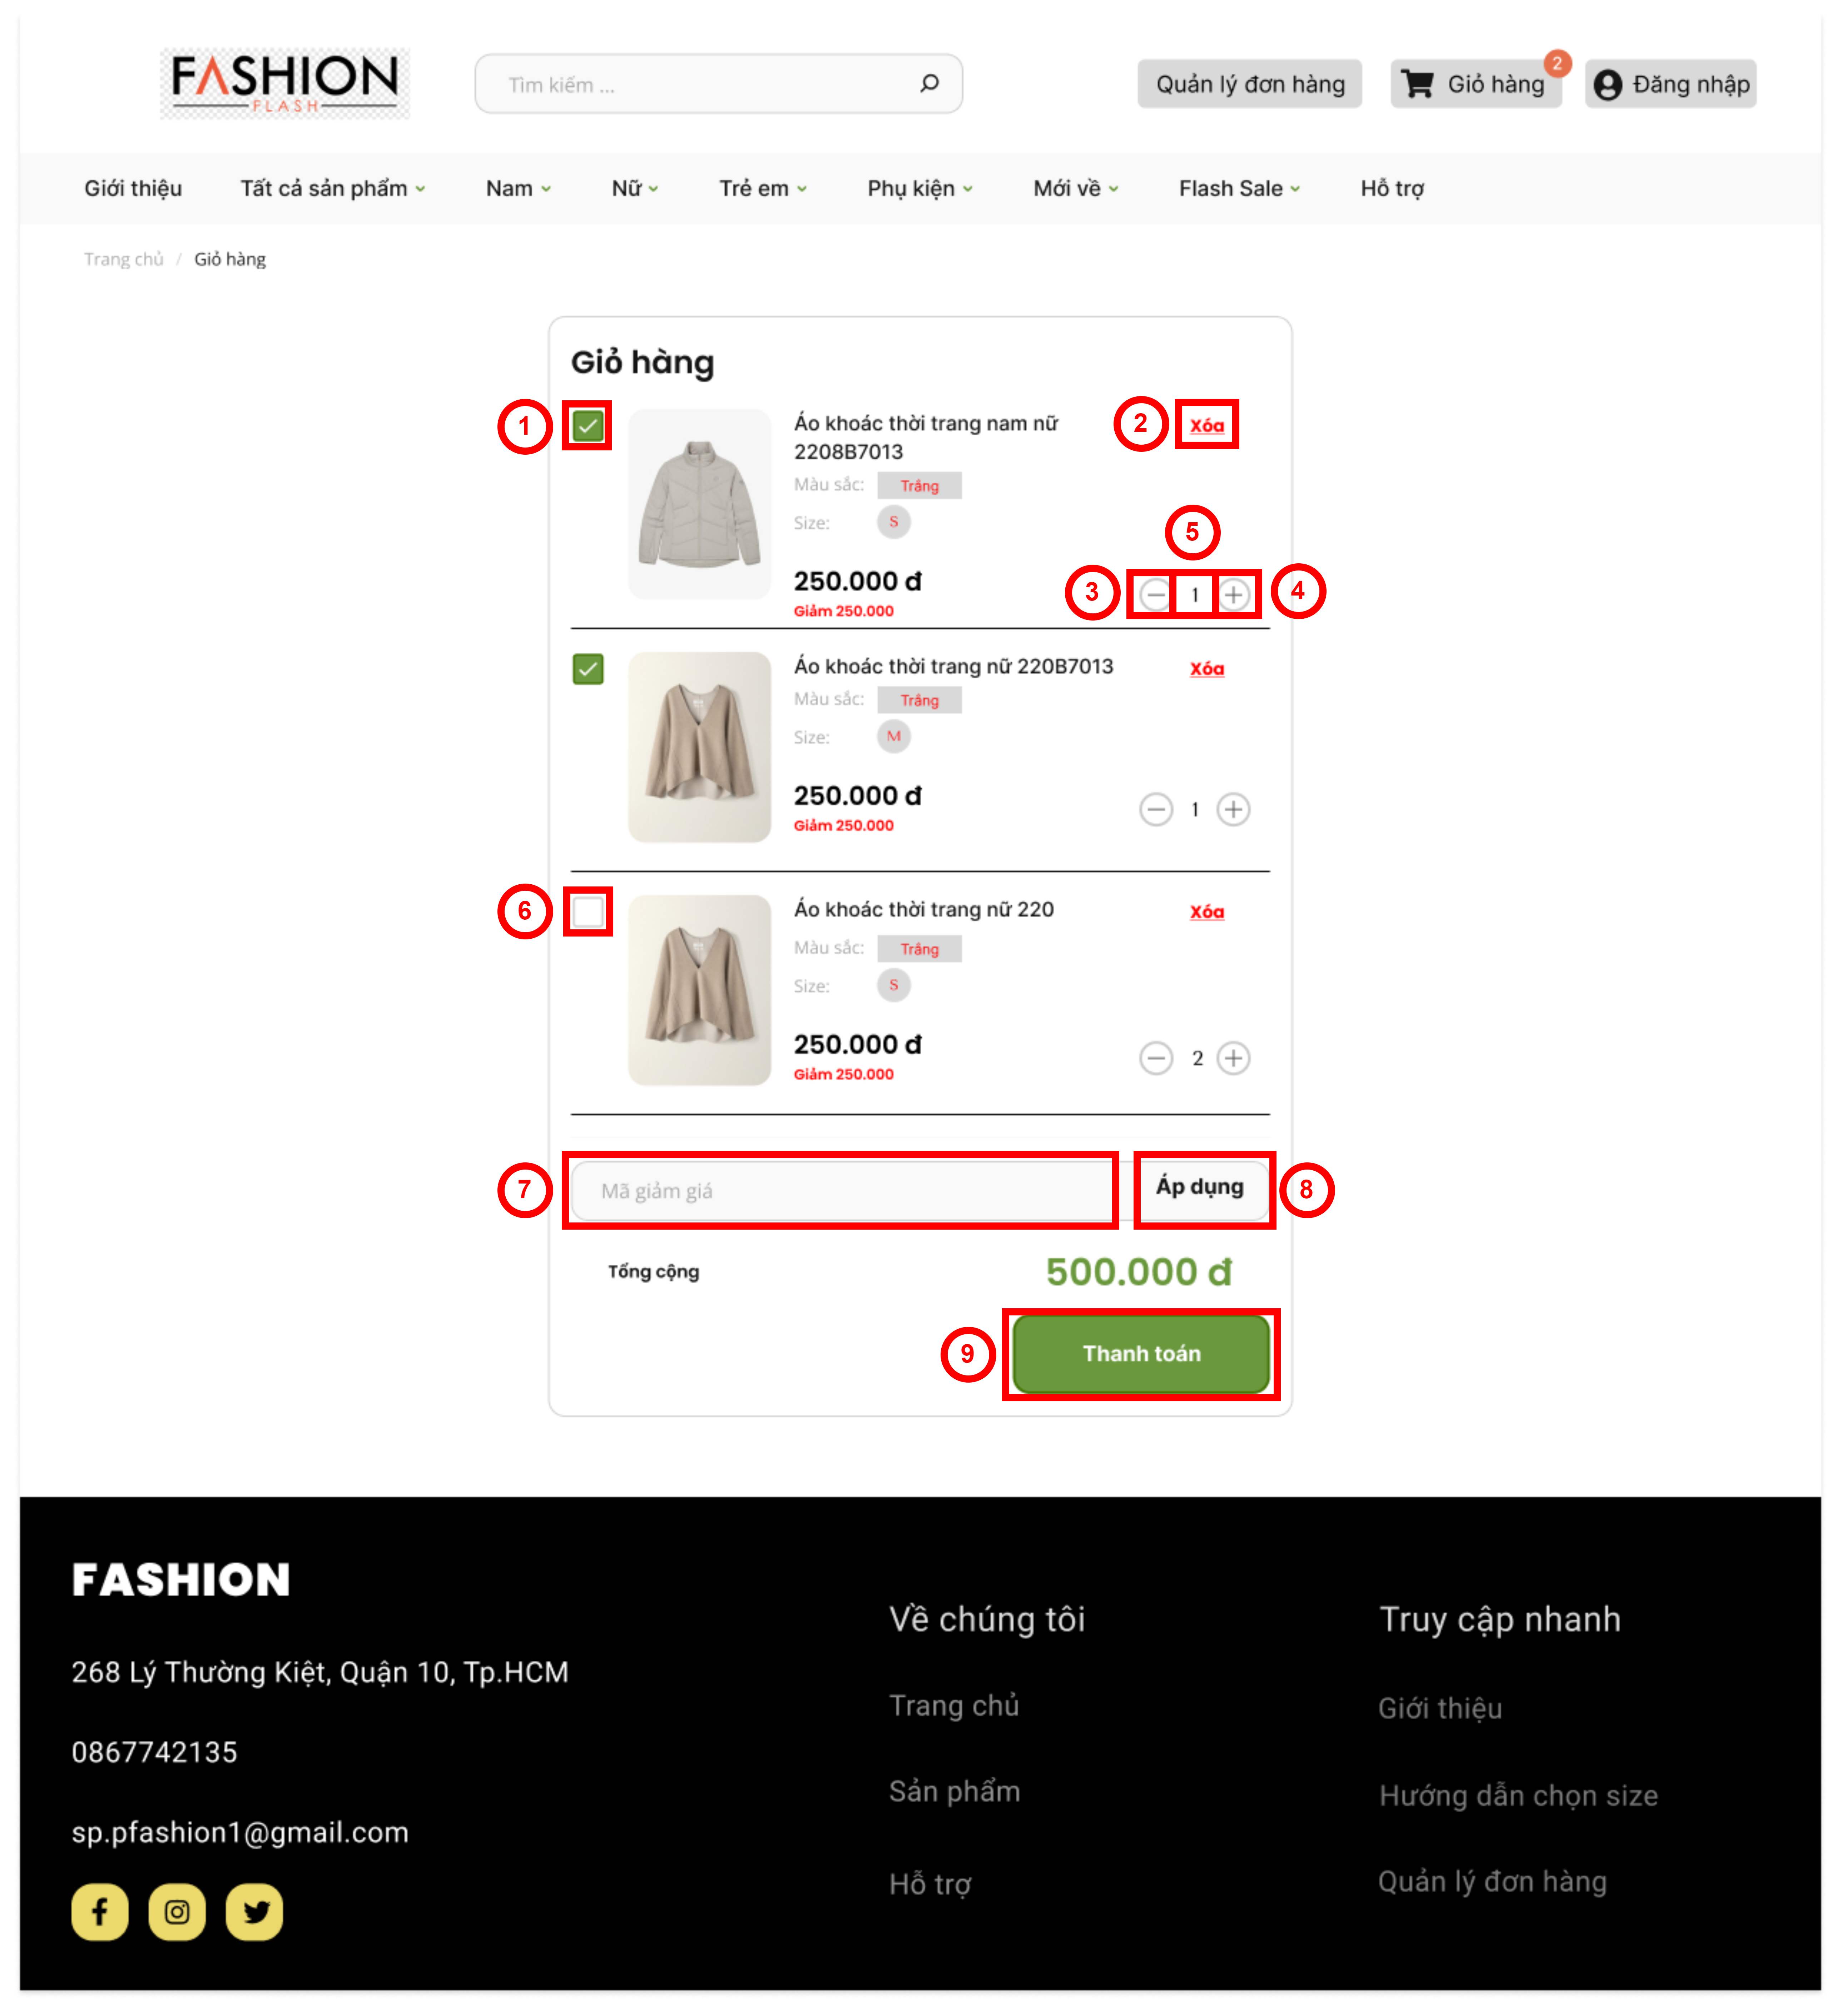
\includegraphics[width=5in]{img/UI/customer/cart.png}
    \label{11}
    \newline
    \caption{Giao diện quản lý giỏ hàng.}
\end{figure}
\textbf{Mô tả:}
\begin{quote}
    \begin{enumerate}
        \item Chọn để loại sản phẩm khỏi danh sách muốn đặt hàng.
        \item Chọn để xóa sản phẩm khỏi giỏ hàng.
        \item Chọn để giảm số lượng mà người dùng muốn.
        \item Chọn để tăng số lượng mà người dùng muốn.
        \item Nhập để thay đổi số lượng mà người dùng muốn.
        \item Chọn để thêm sản phẩm vào danh sách muốn đặt hàng.
        \item Nhập mã giảm giá.
        \item Chọn để áp dụng mã giảm giá.
        \item Chọn để thực hiện thanh toán để đặt hàng.
    \end{enumerate}
\end{quote}
\newpage



\subsubsection{Thanh toán}
\begin{figure}[!htp]
    \centering
    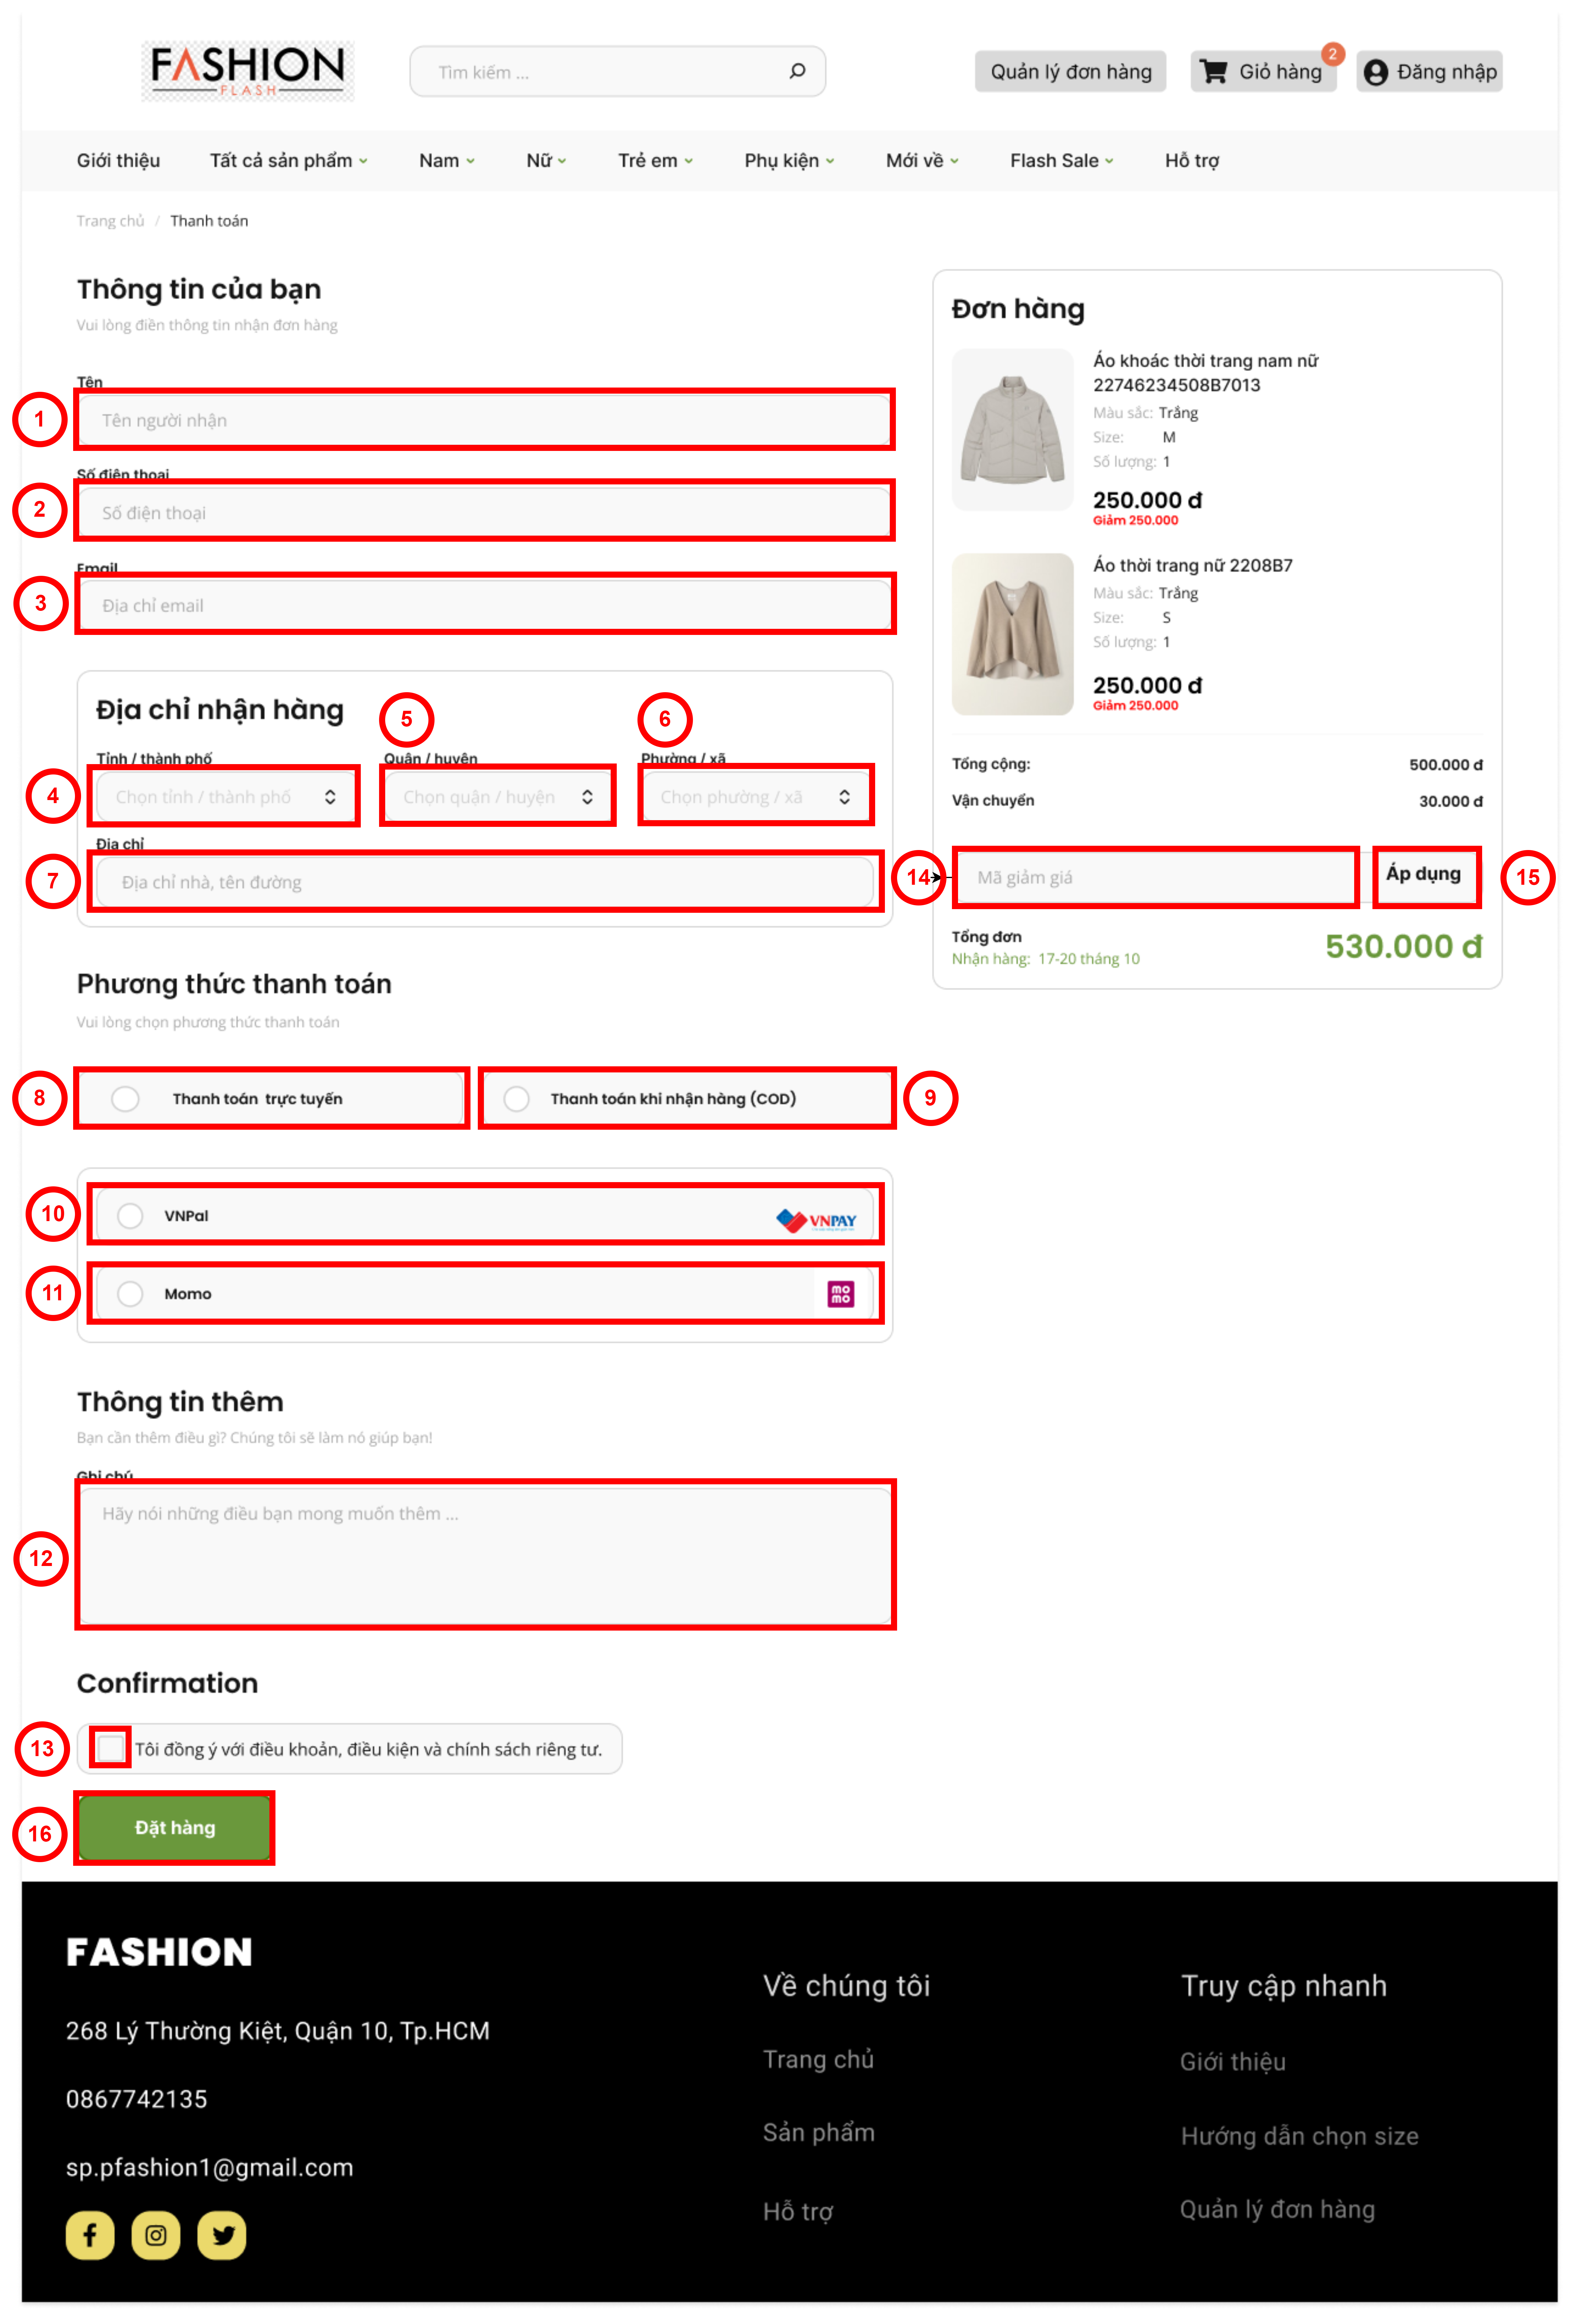
\includegraphics[width=5in]{img/UI/customer/payment.png}
    \label{12}
    \newline
    \caption{Giao diện thanh toán.}
\end{figure}
\textbf{Mô tả:}
\begin{quote}
    \begin{enumerate}
        \item Nhập tên người nhận hàng.
        \item Nhập số điện thoại người nhận hàng.
        \item Nhập địa chỉ email người nhận hàng.
        \item Nhập địa chỉ tỉnh/thành nhận hàng.
        \item Nhập địa chỉ quận/huyện nhận hàng.
        \item Nhập địa chỉ phường/xã nhận hàng.
        \item Nhập địa chỉ số nhà, tên đường nhận hàng.
        \item Chọn để thực hiện thanh toán trực tuyến.
        \item Chọn để thực hiện thanh toán trực tiếp khi nhận hàng.
        \item Chọn để thực hiện thanh toán trực tuyến thông qua VNPay.
        \item Chọn để thực hiện thanh toán trực tuyến thông qua Momo.
        \item Nhập để thêm ghi chú cho đơn hàng.
        \item Chọn để xác nhận đồng ý điều khoản mua hàng.
        \item Nhập mã giảm giá.
        \item Chọn để kiểm tra mã giảm giá và áp dụng giảm giá vào đơn hàng.
        \item Chọn để xác nhận đặt hàng, nếu chọn thanh toán trực tuyến thì sẽ được chuyển đến trang thanh toán của bên thứ ba mà người dùng chọn, nếu chọn thanh toán khi nhận hàng thì đơn hàng sẽ được hoàn tất khi tất cả thông tin hợp lệ.
    \end{enumerate}
\end{quote}

\subsubsection{Giao diện quản lý đơn hàng}
\begin{figure}[!htp]
    \centering
    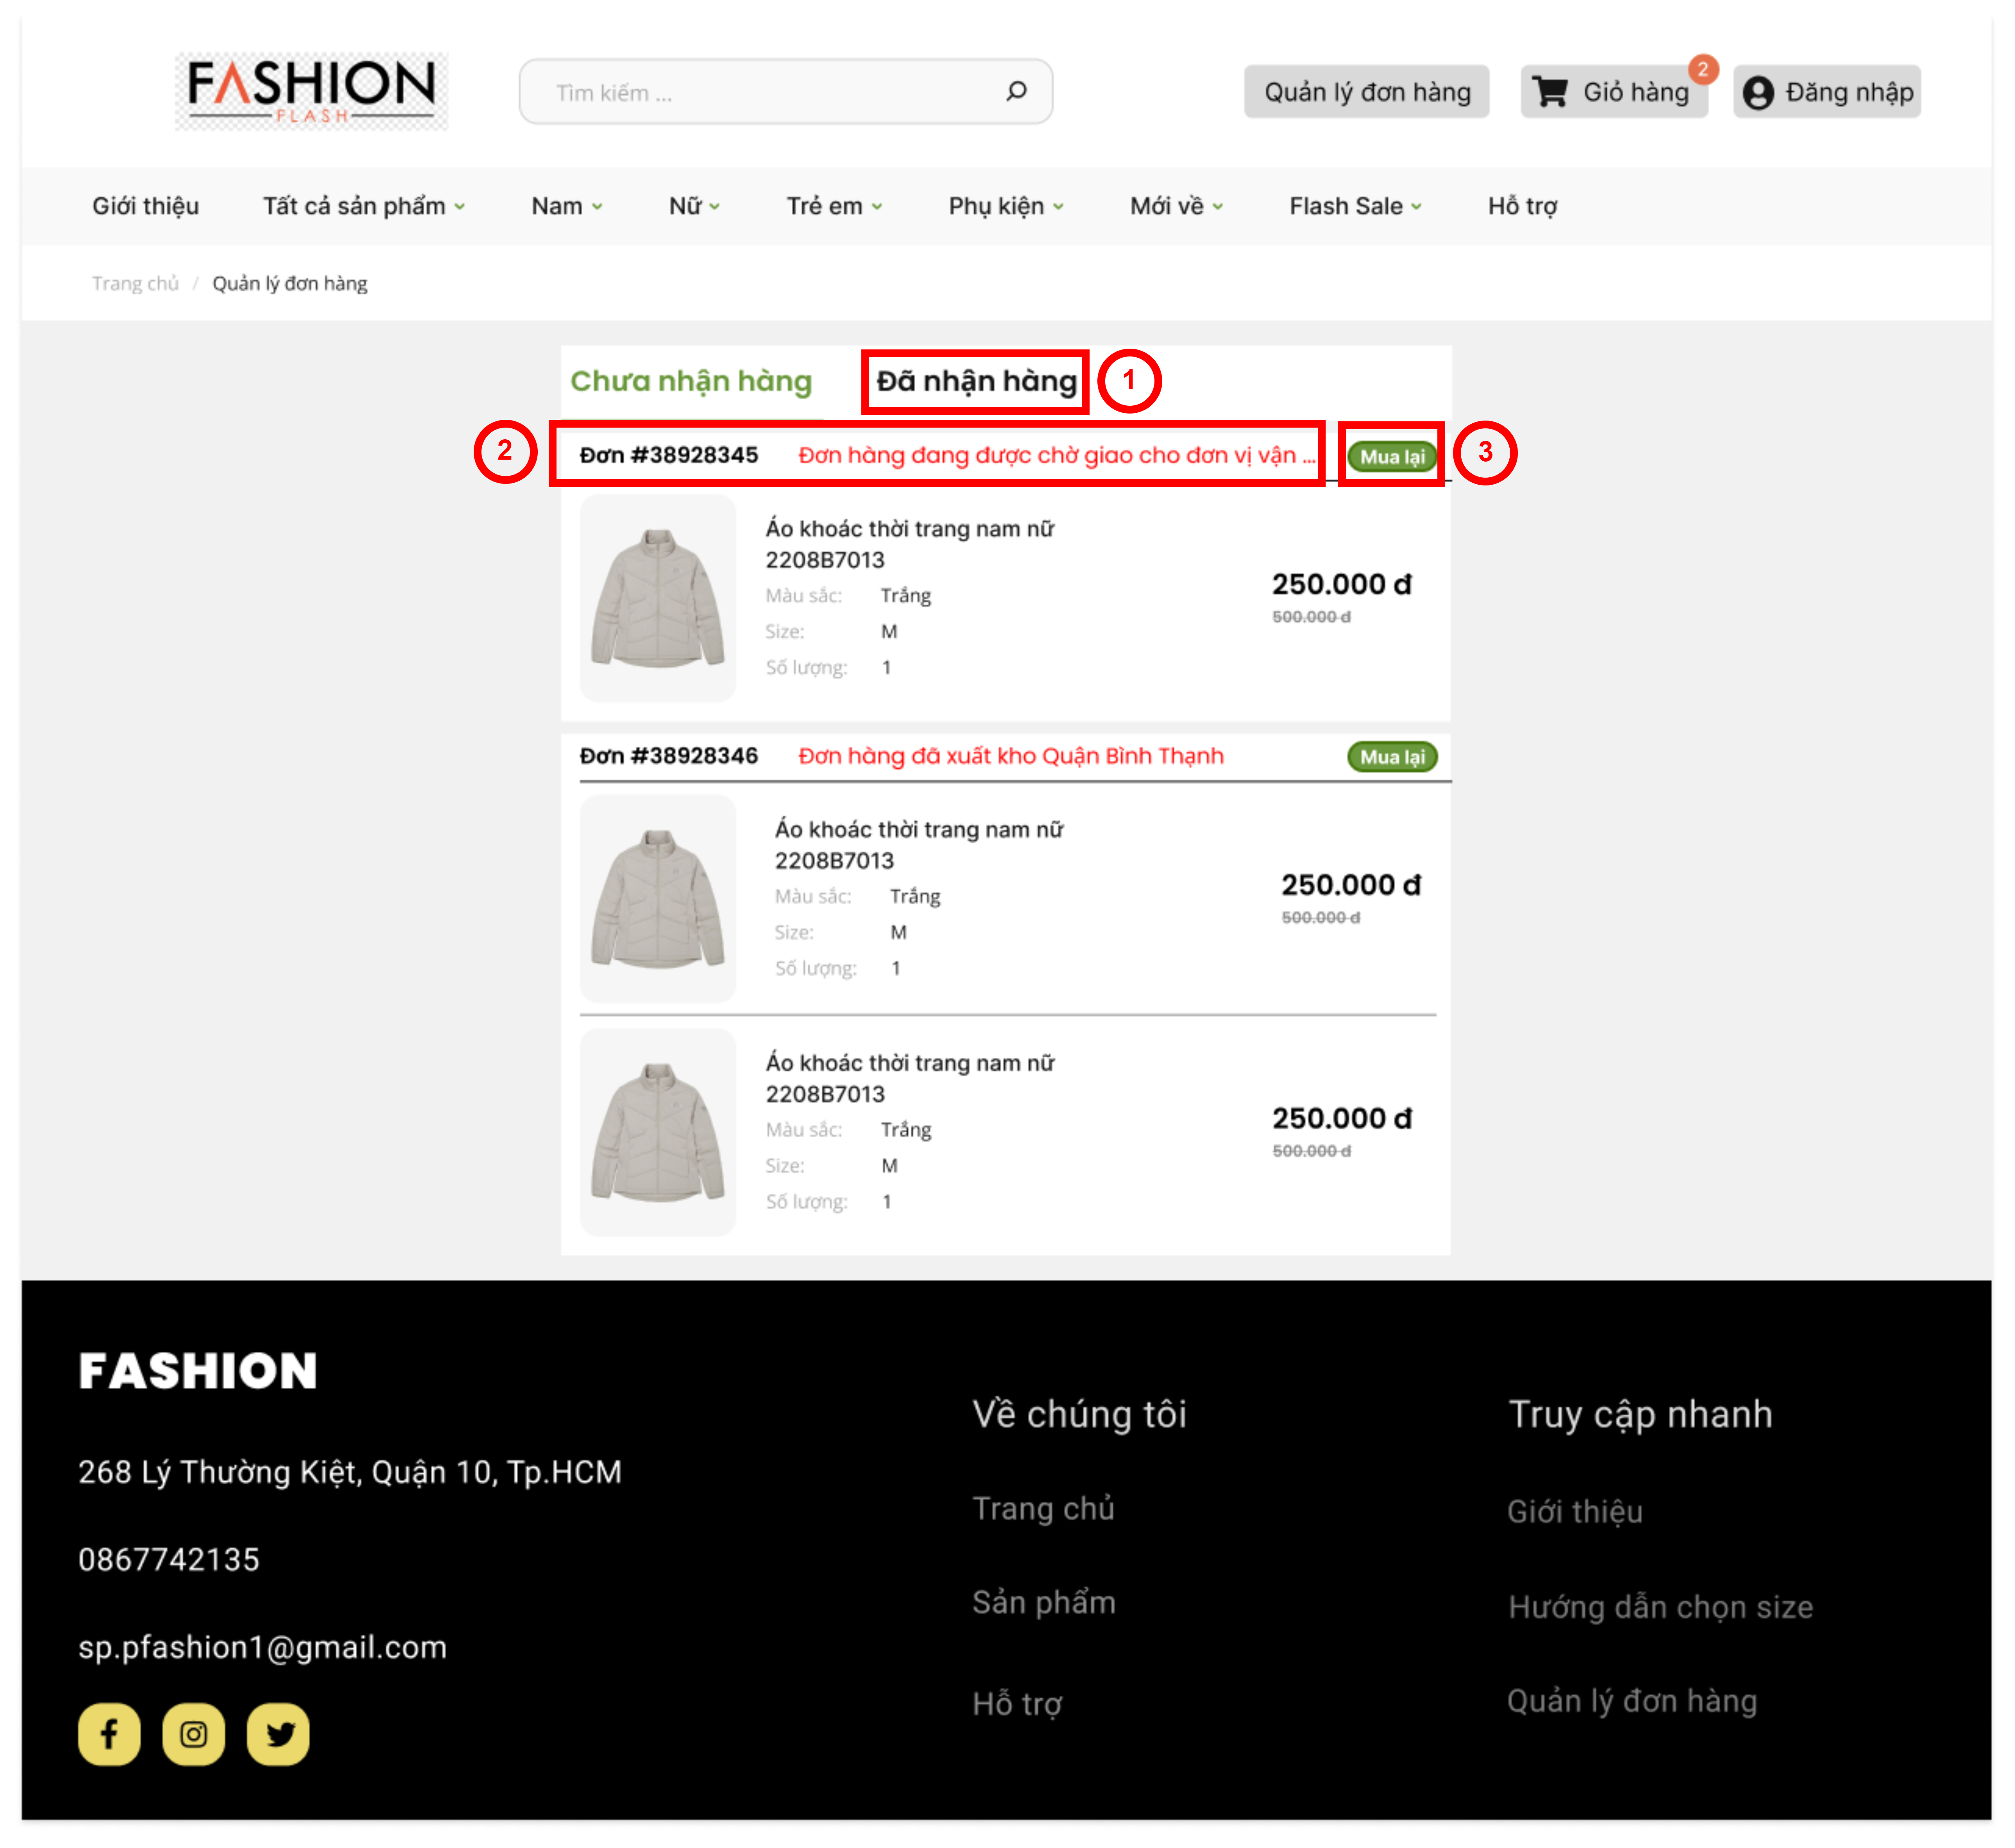
\includegraphics[width=5in]{img/UI/customer/customer_order.png}
    \label{13}
    \newline
    \caption{Giao diện quản lý đơn hàng của khách hàng.}
\end{figure}
\textbf{Mô tả:}
\begin{quote}
    \begin{enumerate}
        \item Chọn để xem danh sách các đơn hàng đã nhận.
        \item Chọn để xem thông tin chi tiết của đơn hàng.
        \item Chọn để thực hiện thêm lại các sản phẩm của đơn hàng vào giỏ hàng.
    \end{enumerate}
\end{quote}

\newpage


\subsubsection{Giao diện chi tiết đơn hàng}
\begin{figure}[!htp]
    \centering
    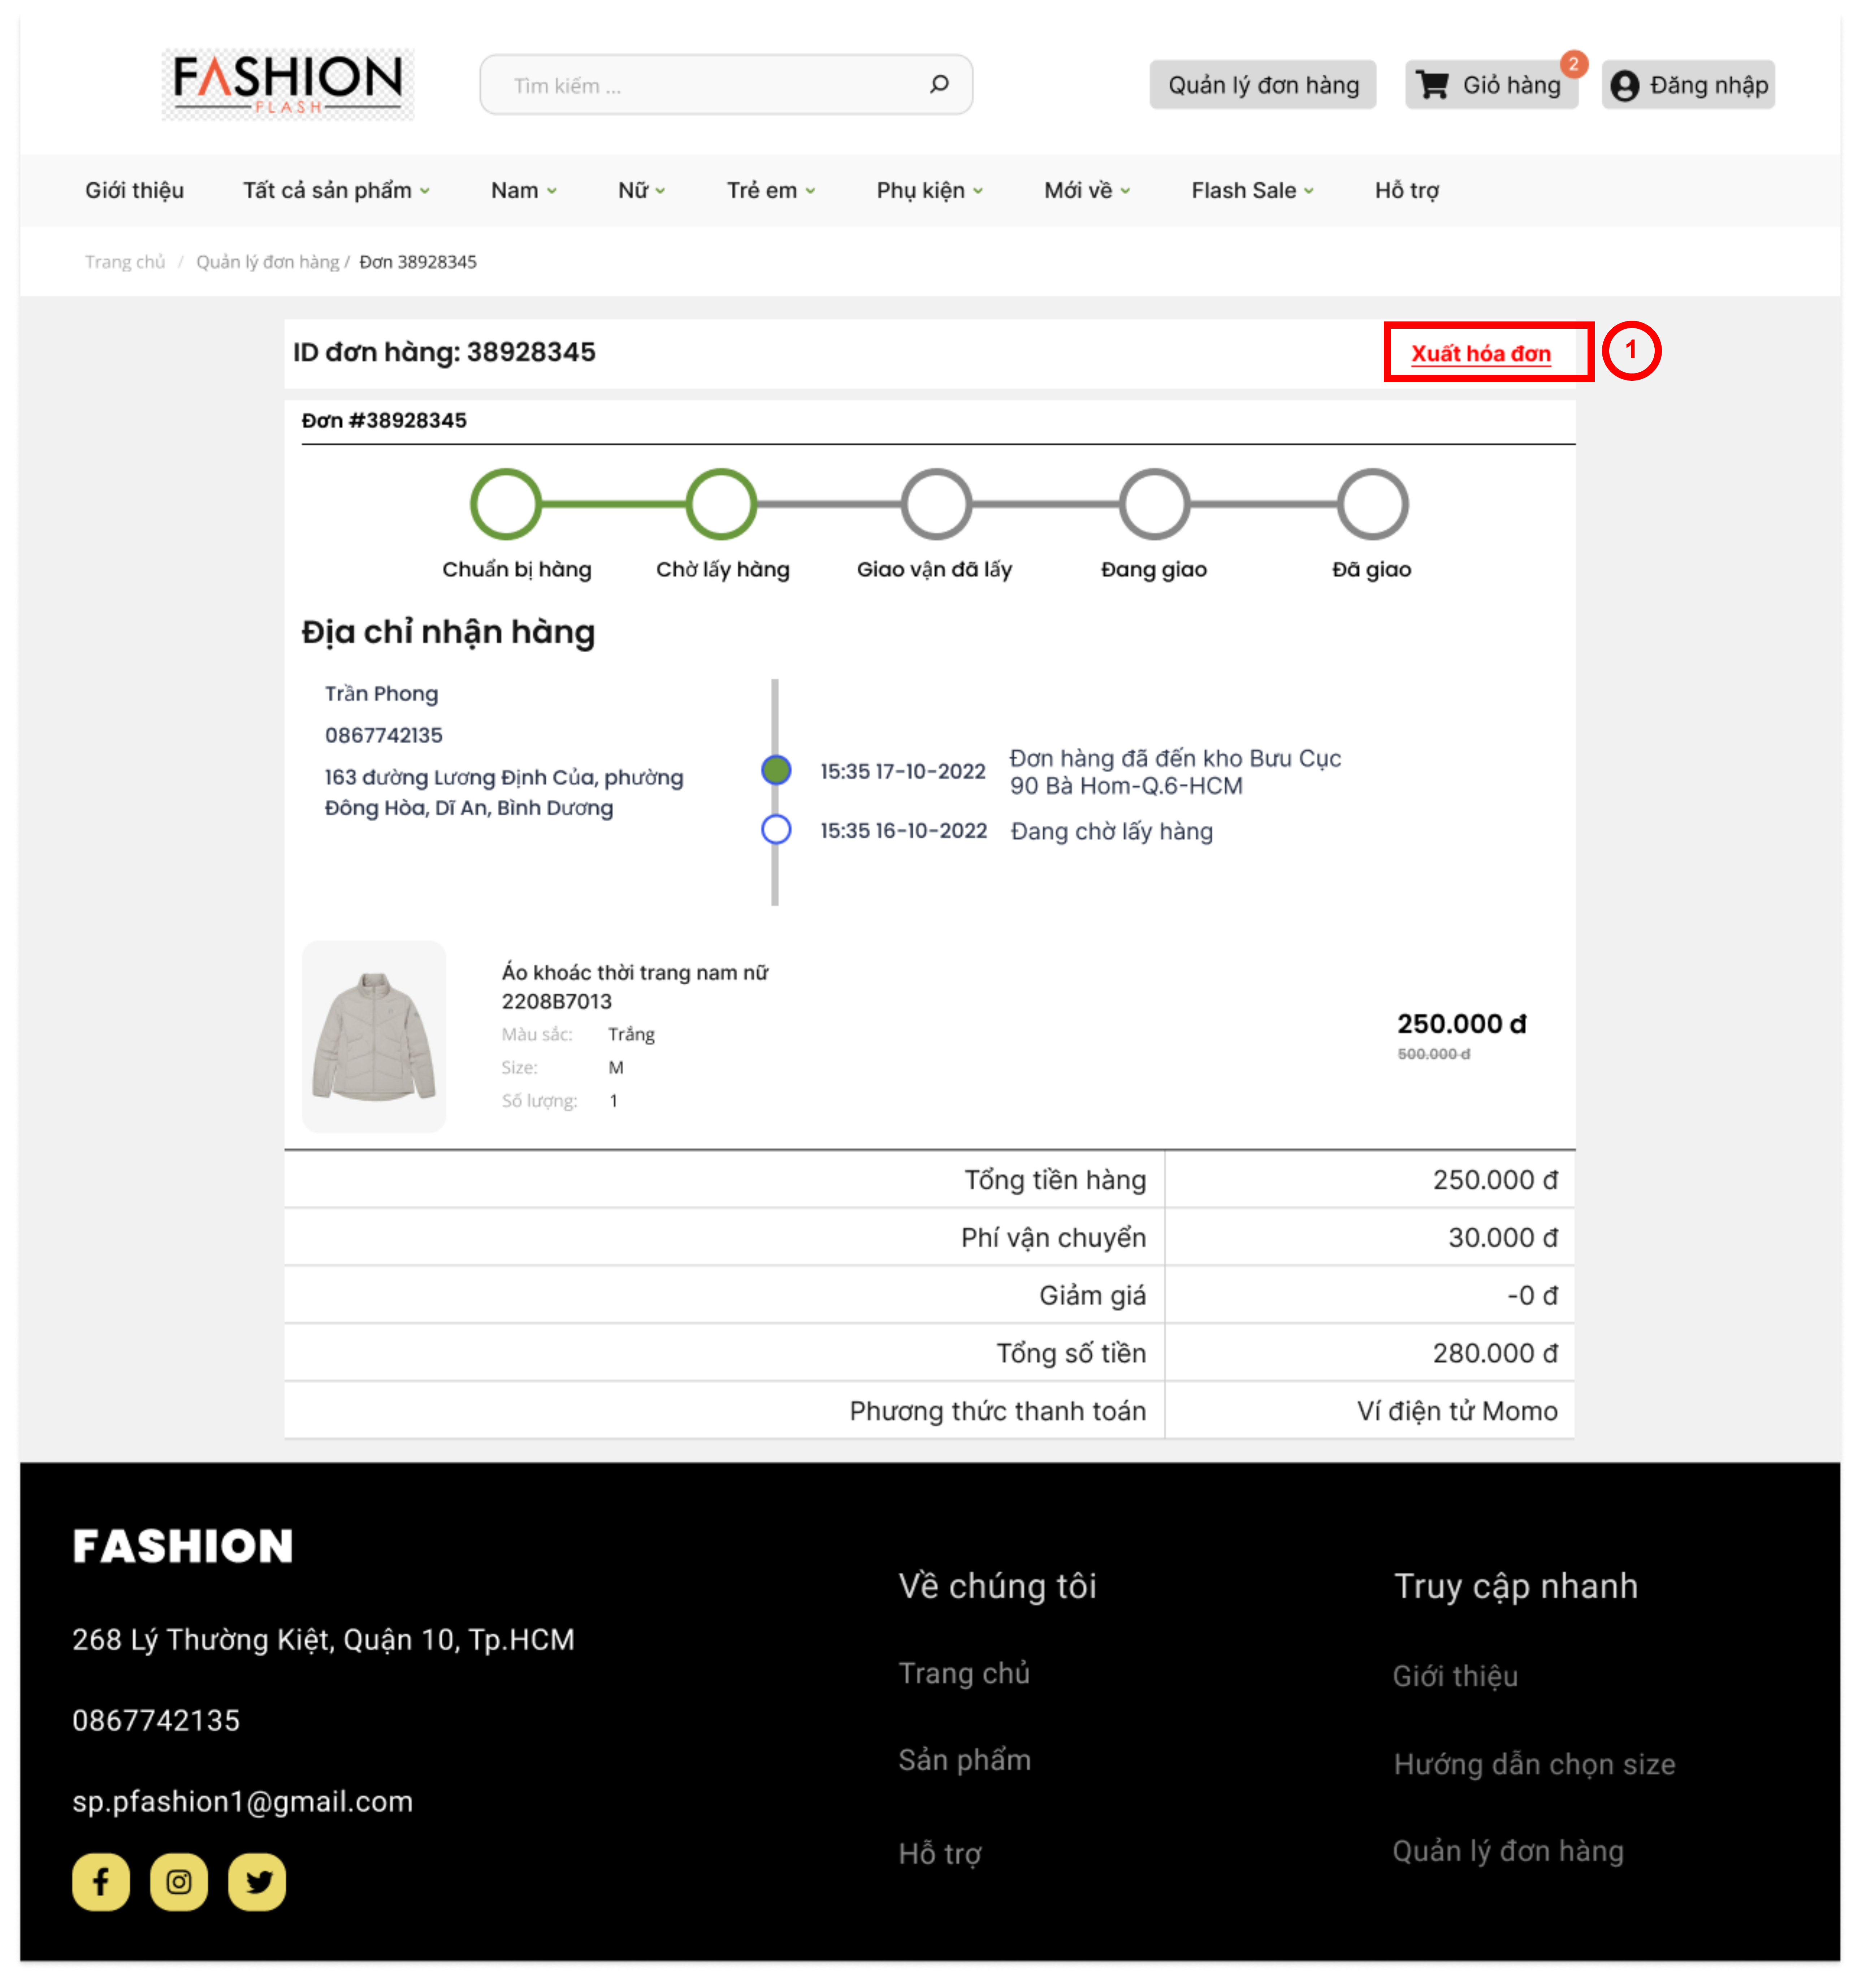
\includegraphics[width=5in]{img/UI/customer/order_detail.png}
    \label{14}
    \newline
    \caption{Giao diện xem chi tiết đơn hàng của khách hàng.}
\end{figure}
\textbf{Mô tả:}
\begin{quote}
    \begin{enumerate}
        \item Chọn để xuất hóa đơn cho đơn hàng.
    \end{enumerate}
\end{quote}

\newpage

\subsubsection{Giao diện thông tin khách hàng}
\begin{figure}[!htp]
    \centering
    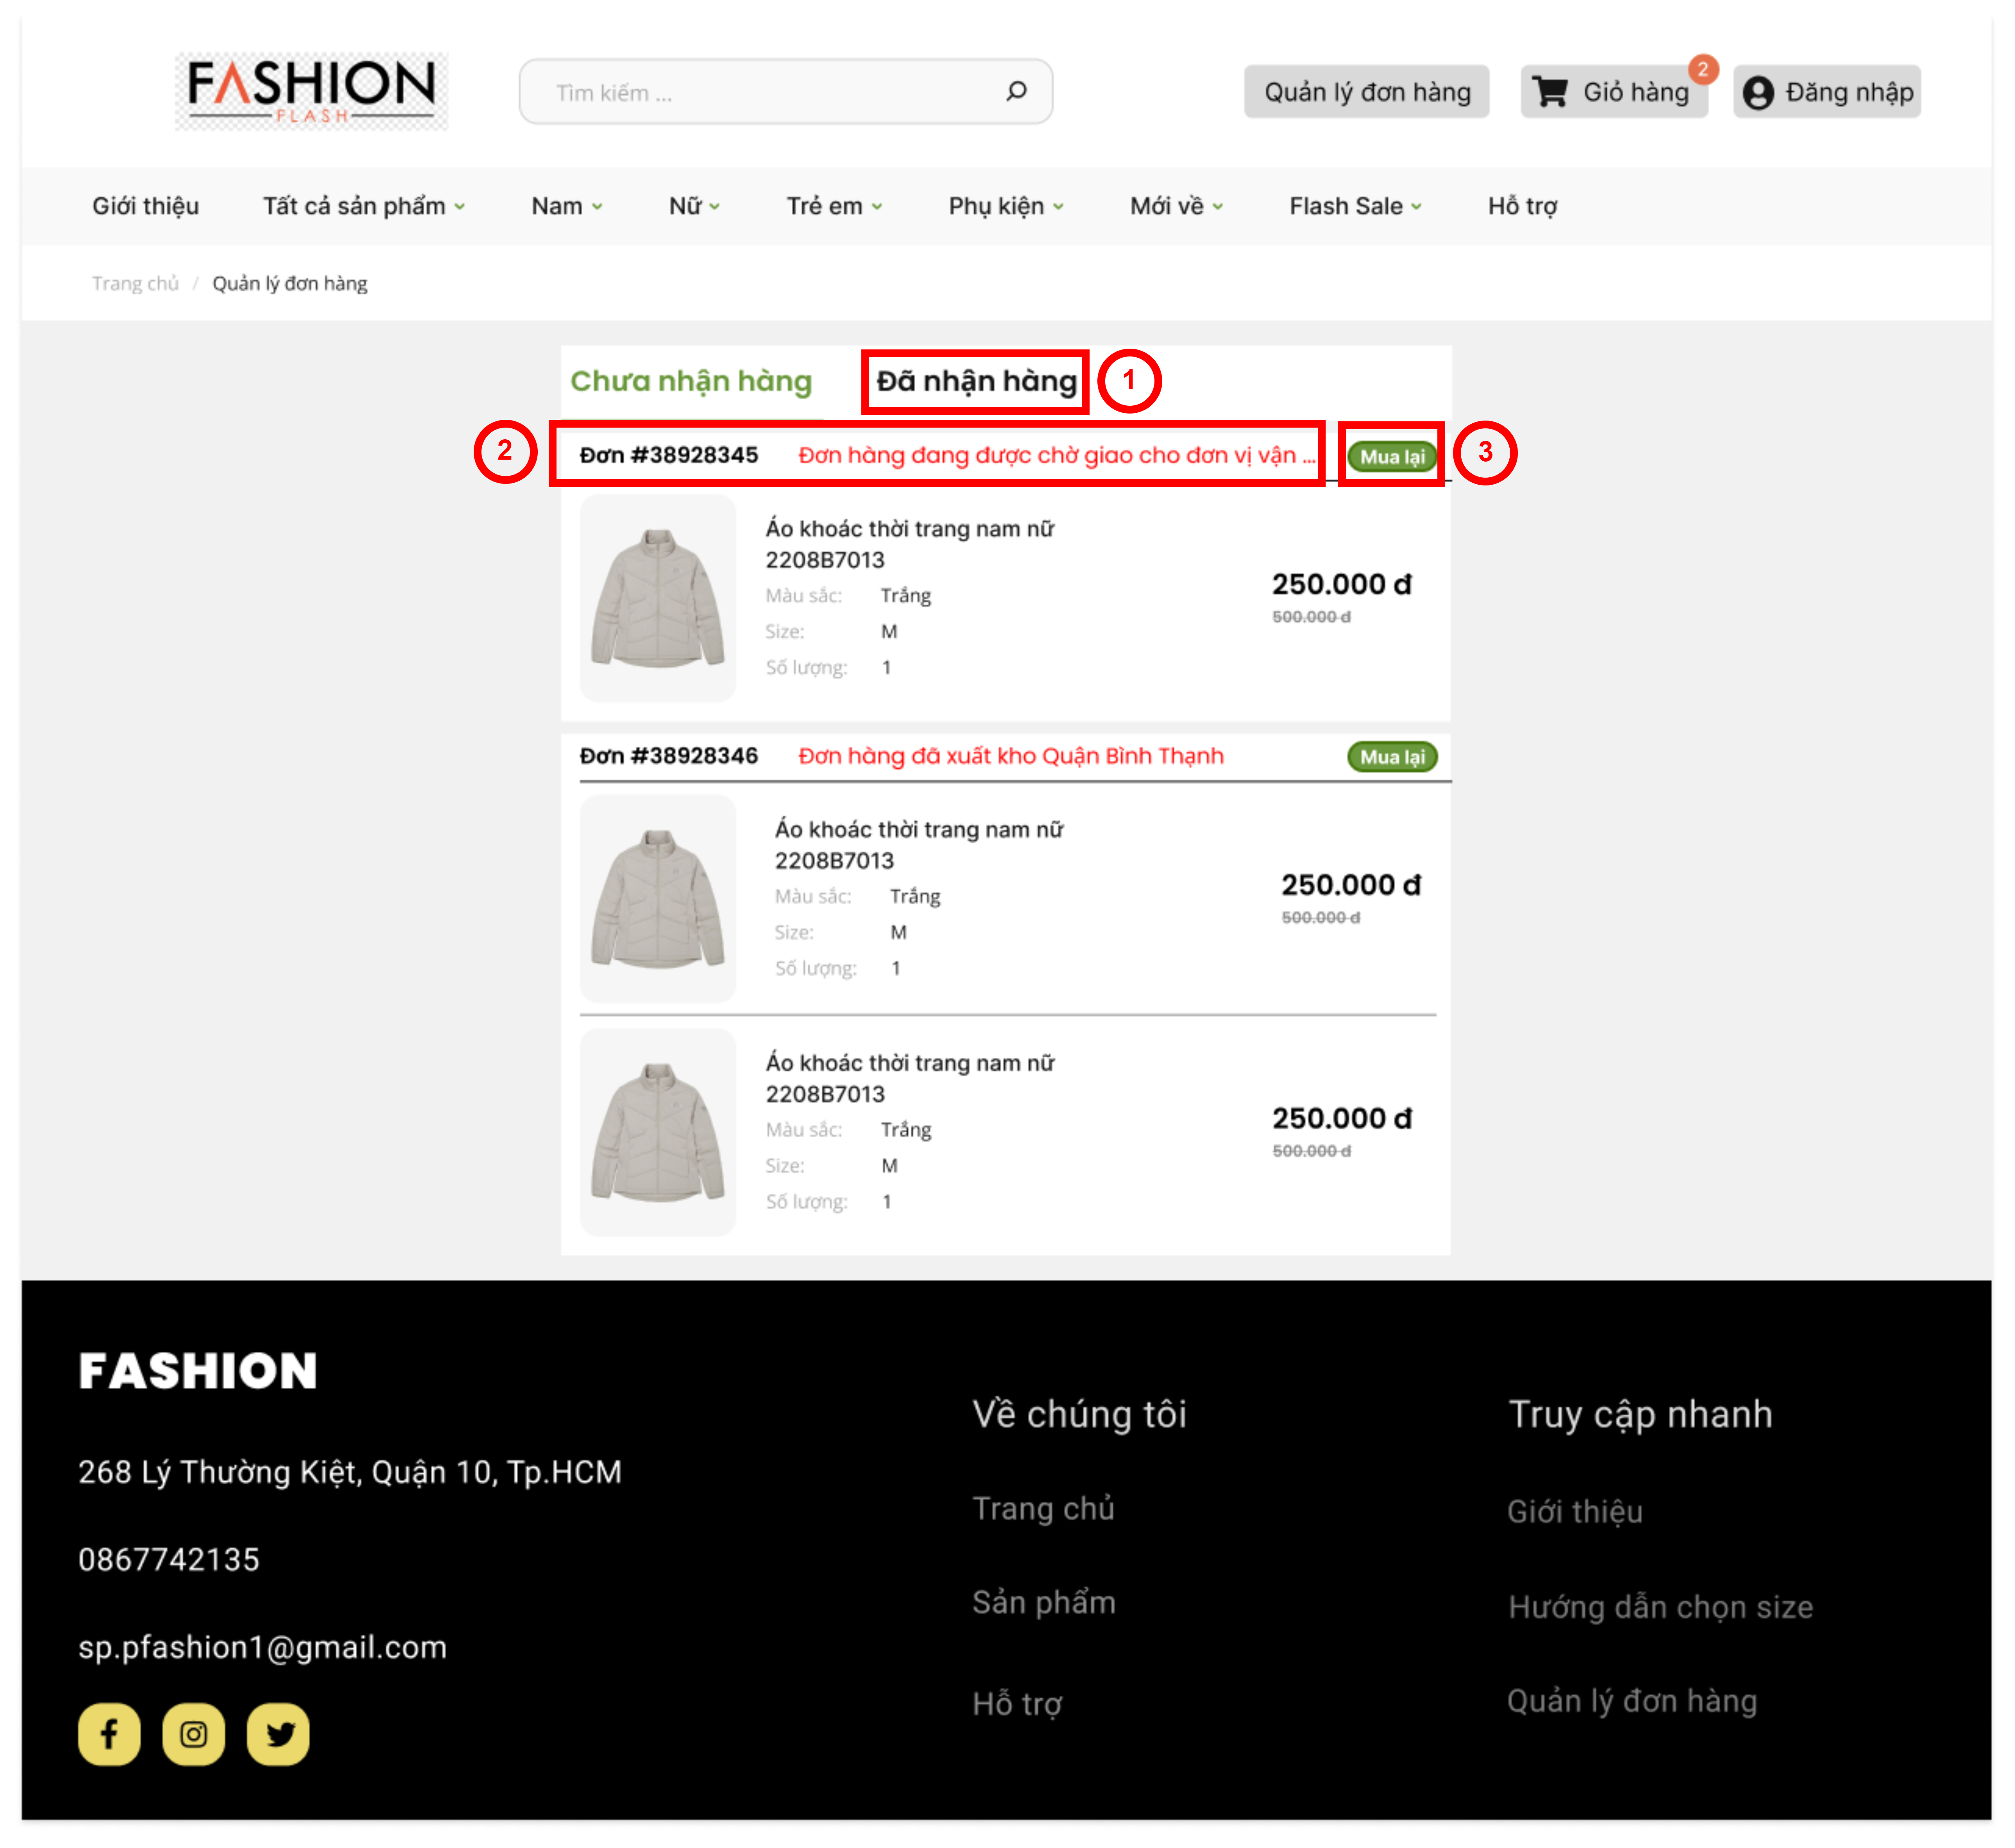
\includegraphics[width=5in]{img/UI/customer/customer_order.png}
    \label{15}
    \newline
    \caption{Giao diện xem thông tin tài khoản của khách hàng.}
\end{figure}
\textbf{Mô tả:}
\begin{quote}
    \begin{enumerate}
        \item Nhập để thay đổi tên của khách hàng.
        \item Nhập để thay đổi email của khách hàng.
        \item Chọn để thực hiện thay đổi mật khẩu của khách hàng.
        \item Nhập để thay đổi số nhà, đường của địa chỉ mặc định mà khách hàng muốn nhận hàng.
        \item Chọn để thay đổi phường/xã của địa chỉ mặc định mà khách hàng muốn nhận hàng.
        \item Chọn để thay đổi quận/huyện của địa chỉ mặc định mà khách hàng muốn nhận hàng.
        \item Chọn để thay đổi tỉnh/thành phố của địa chỉ mặc định mà khách hàng muốn nhận hàng.
        \item Chọn để thay đổi ảnh đại hình cho tài khoản của khách hàng.
    \end{enumerate}
\end{quote}

\newpage

Giao diện sau khi chọn "Đổi mật khẩu":
\begin{figure}[!htp]
    \centering
    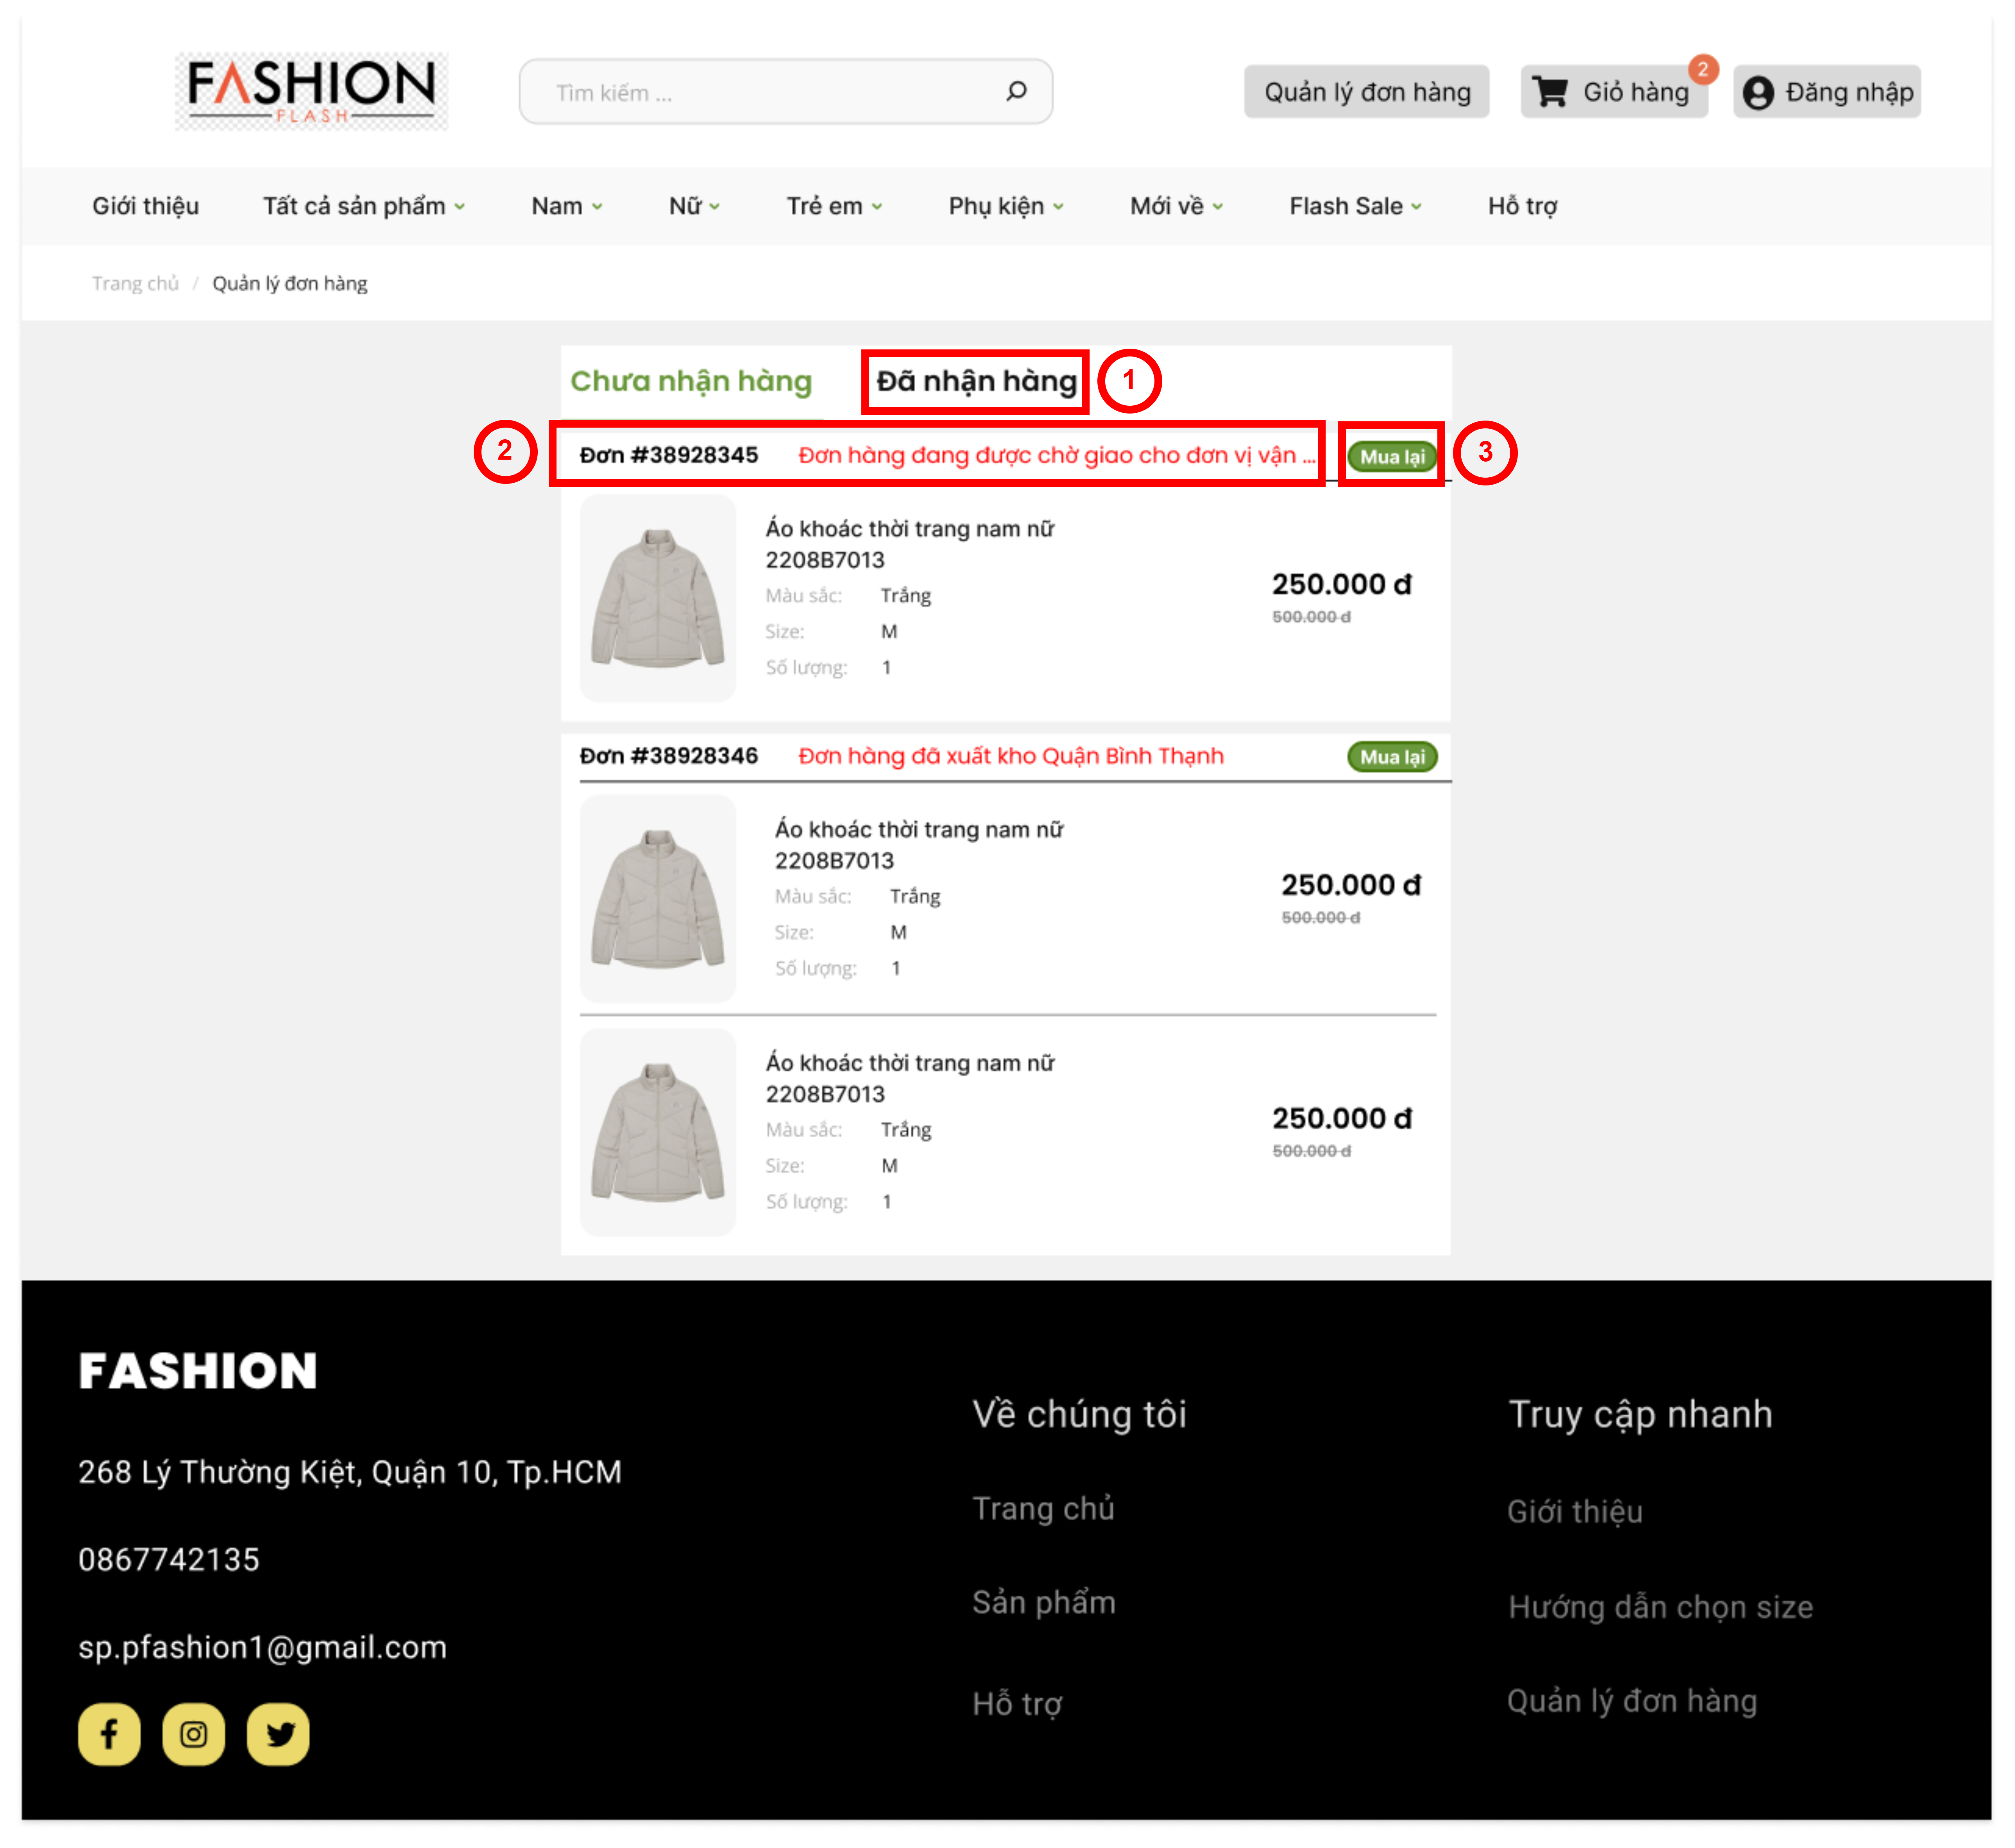
\includegraphics[width=5in]{img/UI/customer/customer_order.png}
    \label{16}
    \newline
    \caption{Giao diện đổi mật khẩu cho tài khoản.}
\end{figure}

\textbf{Mô tả:}
\begin{quote}
    \begin{enumerate}
        \item Nhập để điền mật khẩu cũ, yêu cầu tối thiểu 6 ký tự.
        \item Nhập để điền mật khẩu mới, yêu cầu tối thiểu 6 ký tự.
        \item Nhập để điền xác nhận mật khẩu mới, yêu cầu giống mật khẩu mới.
        \item Chọn để xác nhận thay đổi mật khẩu.
        \item Chọn để tắt màn hình khi không muốn thay đổi mật khẩu nữa.
    \end{enumerate}
\end{quote}

\newpage

